\setcounter{mtc}{5}
% see https://tex.stackexchange.com/questions/36846/minitoc-thesis-template-pdflatex for the use of setcounter for minitoc in this context.


\chapter{Preparing the ground}
\emph{`...there is nothing new under the sun. \\Is there anything of which one can say,``Look! This is something new"?'}~\footnote{\href{https://www.biblegateway.com/passage/?search=Ecclesiastes+1\%3A9-10&version=NIV}{Ecclesiastes Ch:1 vv. 9-10 NIV edition.}}

\vspace{10mm}

This chapter provides a grounding in the domain of mobile apps, how developers obtain information, and mobile analytics,~\emph{etc.}  
% MUST-DO revise opening sentence and remove the etc. via \akb
For any individual elements there may be much that is known and seemingly little novelty. And yet, it has become clear that when these elements are combined an interesting and rich domain emerges that can serve developers of their mobile apps.

Before diving into the rest of the chapter, please note, 
there are limits of the certainty of closed, proprietary systems including those discussed in this thesis. Therefore, there may be situations where there are differences between these observations and findings and those of other users of these tools. To improve readability the thesis includes some generalisations rather than using qualifiers throughout, such as often, mainly, and so on, unless they materially reflect variations in people's experiences.

The chapter introduces five 
%MUST-DO revise this and the next paragraph once the chapter's contents have settled down.
conceptual models, including: a model of apps and app stores, layers of an app and observation points, of analogue and digital feedback, usage analytics, and finally DevOps. These concepts help us understand key considerations for mobile app developers and what they are working with.

The chapter continues with five practical aspects including app development and usage, information sources for developers, and choices for engaging with analytics. Developers need to address these as part of being effective in their work and providing apps of adequate quality. Mobile analytics can provide useful sources of information, including problems with the apps in use, and mobile analytics can complement and calibrate other sources of quality related information including software testing. 

\begin{comment}
% See also https://tex.stackexchange.com/questions/3001/list-sections-of-chapter-at-beginning-of-that-chapter
\minitoc 
\mtcskip 
\setcounter{mtc}{4} %This is a hack as minitoc seems to have different counters for the toc and the figures. As I'm probably only using minitoc temporarily while working on the chapter I can live with this. See https://tex.stackexchange.com/questions/184135/adding-general-introduction-to-table-of-contents-as-chapter-causes-a-problem to try and align the counters, I parked this issue as not worth the time investment currently. 
\minilof
\end{comment}

\section{Development practices for mobile apps}
Few if any developers write perfect software, and this applies also to developers of mobile apps. 

%SHOULD-DO Add the Amphitheatre illustration. And suitable words to explain the concepts.

This section introduces the concept of \textit{Zones} as they apply to finding and potentially fixing issues while developing software. The concepts are inspired by various sources including agile development practices, release management for mobile apps, computer networks, and particularly the use of firewars and `de-militarised-zones' (known as DMZ). 

\subsection{Control (find-fix) zones}
A find-fix Zone incorporates the scope of finding issues and being able to fix, or at least ameliorate, them. Where issues are discovered in the local Zone, developers can fix the issue without needing to involve others (however they can choose to do so), and indeed some may consider these issues an intrinsic and essential part of iterative software development. Other zones extend beyond the immediate developer and involve other people.

For the purposes of my research I propose three categories of zones:
\begin{enumerate}
    \item \textbf{Local Zone}: This is local to the developer of software, tests, resources, designs, and so on.
    \item \textbf{Mezzo Zone(s)}: These zones involve other people, they may be peers, team members, other people in the organisation, trusted testers, and so on. There may be anything from virtually no zone for solo independent developers working on their own app, to a plethora of zones involving various stages of pre-release testing, checking and approvals in large corporate organisations.
    \item \textbf{Live Zone}: End users are able to use the released app. The app is finally able to potentially achieve business objectives. 
\end{enumerate}



\begin{figure}[htbp!]
    \centering
    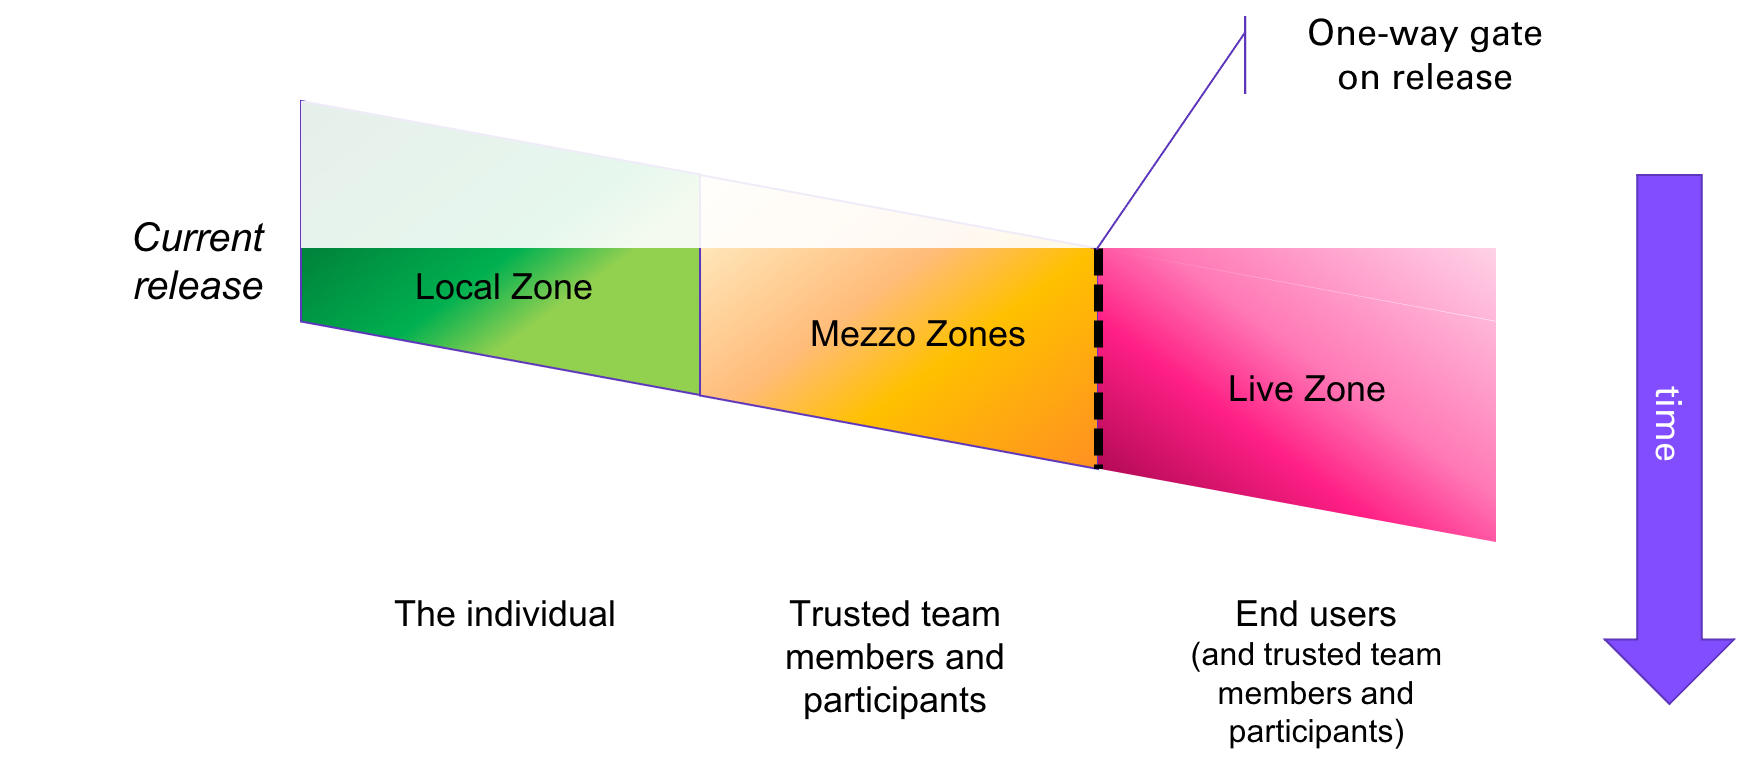
\includegraphics[width=13cm]{images/my/control-find-fix-zones-a.png}
    \caption{Control find-fix zones}
    \label{fig:my:control-find-fix-zones-overview}
\end{figure}

These three categories of zones are illustrated in Figure~\ref{fig:my:control-find-fix-zones-overview}. The figure includes a one-way gate, that behaves like the Rubicon in Julius Caesar's time~\citep{wikipedia_rubicon} where the die is cast once a release has been launched in the app store. The release cannot be reverted, at best it can be paused or superseded with another subsequent release. The app now comes into contact with end-users and is expected to achieve the business objectives of the organisation who made it available.

\begin{figure}[htbp!]
    \centering
    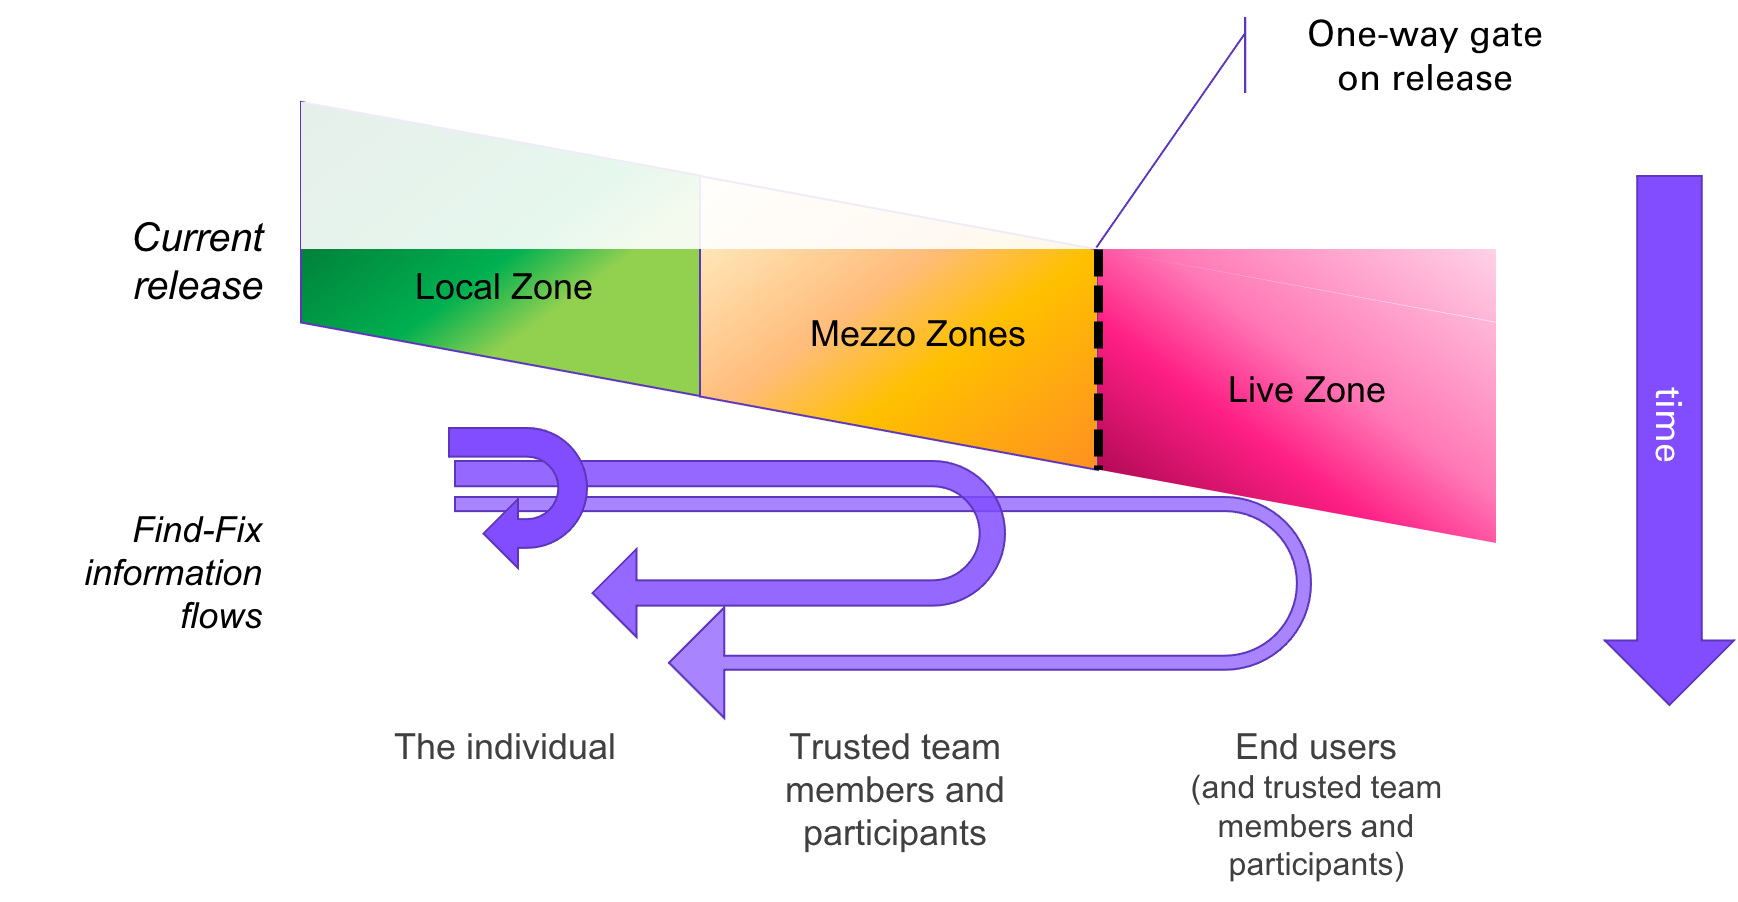
\includegraphics[width=13cm]{images/my/control-find-fix-zones-with-information-flows.png}
    \caption{Control find-fix zones with information flows}
    \label{fig:my:control-find-fix-zones-with-information-flows}
\end{figure}

Figure~\ref{fig:my:control-find-fix-zones-with-information-flows} is a modified version of Figure~\ref{fig:my:control-find-fix-zones-overview} that includes the find-fix information flows. Assuming fixes are made be the development team for the app (rather than improvements that can be addressed in servers, through configuration changes, and so on) then the information about flaws and issues needs to reach that development team somehow. For issues found in external releases (\emph{i.e.} those made available to end-users) 


When issues are discovered before the software is released there is the possibility of the developer being able to address them before the software is released (they stakeholders may choose to delay the release to allow this to happen). Where issues are discovered in the released app, unless there are viable mechanisms to patch the app, the fix needs to be made in a subsequent release \textit{and} the end-user needs to use the subsequent release to receive the benefit of the release.

There are two key challenges:
\begin{enumerate}
    \item the developer learning about issues in sufficient detail to potentially address them,
    \item being able to address issues and provide the benefit to users who are, or  may be, affected by it.
\end{enumerate}

Both these aspects are covered next in terms of the bug-fix process for mobile apps.

\subsection{Bug-fix process for mobile apps}
%MUST-DO move the following comment to the next chapter once I've drafted the relevant illustrations.
% In my view, mobile analytics helps in the 'current' timeframe of the development and release process, in that it can provide ranked notifications of various issues (including 'stability' failures: i.e. crashes and ANRs) on a timely basis. 

Given apps have been released and users are using those releases then - there may be issues in the app exposed while it is in-use. Some of these may be noticeable (or perceivable) by the end-users, others not. These issues include 'stability' failures: \textit{i.e.} crashes and ANRs and performance-related issues \textit{e.g.} slow responses, excessive power and network consumption, and so on.

For the development team to actively address any of these failures they need to be aware of them and have sufficient details to take action. Figure~\ref{fig:my:bug-fix-process-for-mobile-apps-in-prod} illustrates past, current, and future, activities for current and future releases of an app. We will return to this figure %in this section and 
in the next chapter where the effects of applying analytics to the development process is considered.
%MUST-DO make sure I do return to {fig:my:bug-fix-process-for-mobile-apps-in-prod} in the next chapter, on applying analytics.

\begin{figure}[!htbp]
    \centering
    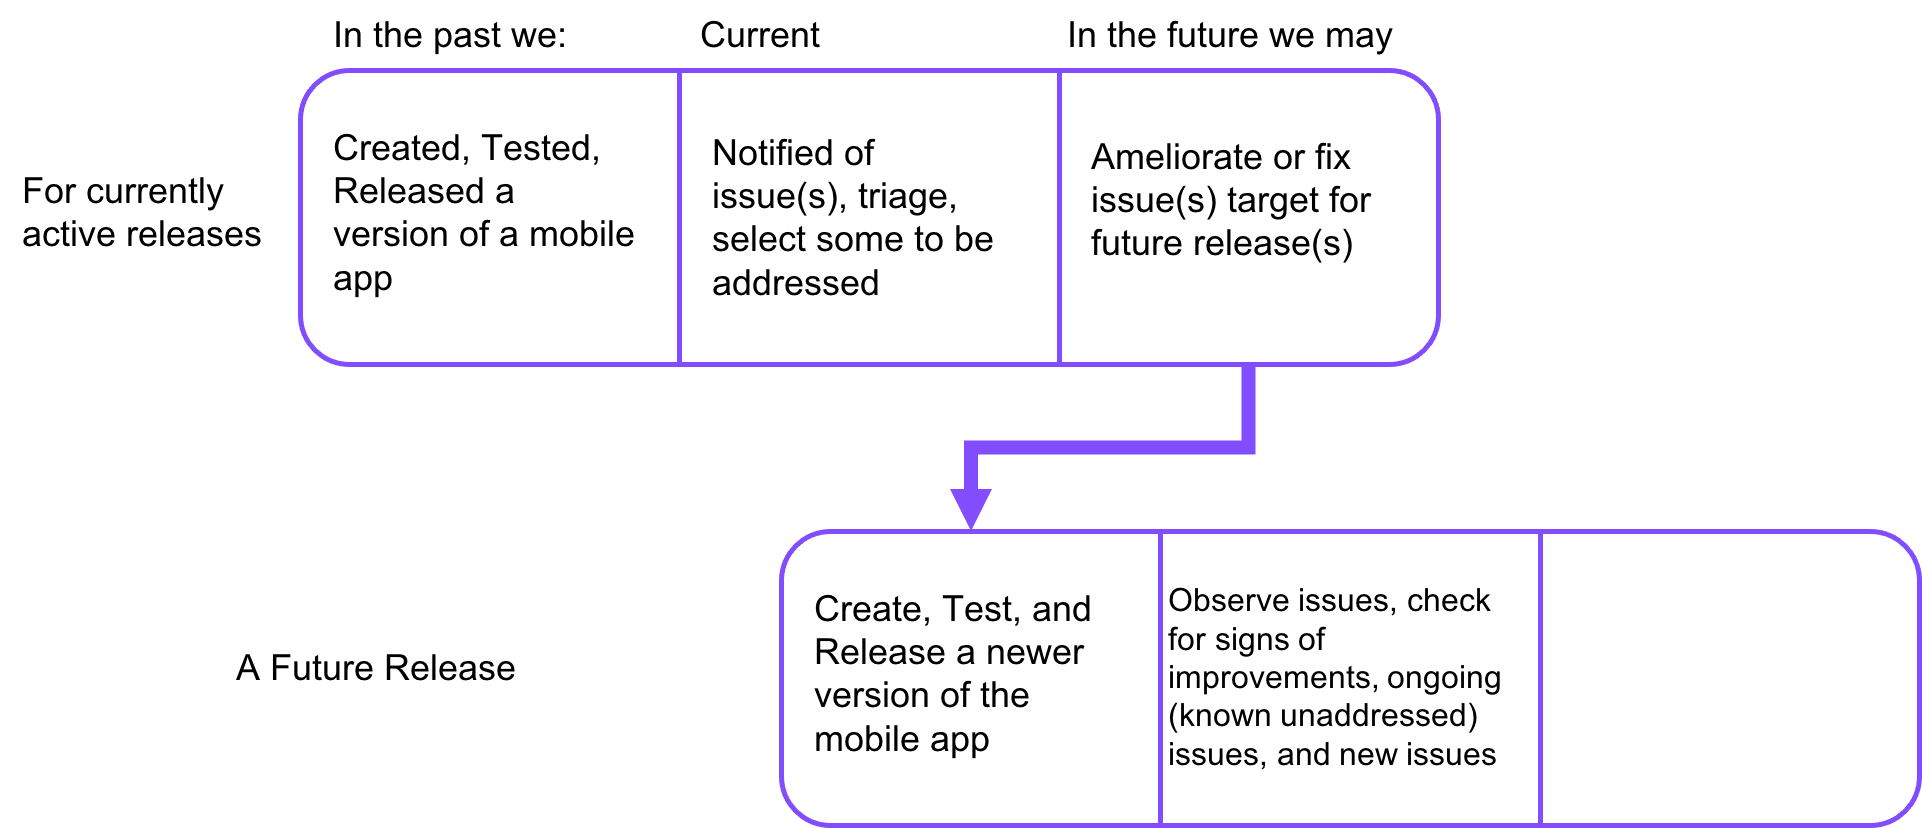
\includegraphics[width=13cm]{images/my/production-bug-fix-process-for-mobile-apps.png}
    \caption{Bug-fix, process for mobile apps in production}
    \label{fig:my:bug-fix-process-for-mobile-apps-in-prod}
\end{figure}


Developers might learn of some of these issues from other sources e.g. from colleagues who use the app, from end-users who report issues (e.g. in reviews in the app store, on social-media, and even using in-app feedback if the app's functioning sufficiently etc.). 
% MUST-DO refer to research in automatically creating automated tests to reproduce crashes and discuss some of the limitations of that research vector. Note: this might be covered in the related works chapter.
However in my experience, and based on other research, only a subset of the issues are reported by people who use the app, and certainly not all users report all the stability issues all of the time.

Any amelioration or fix that occurs in the app's codebase is only useful to those users who use the newer release of the app that include the improvements. Our research confirms some users continue using older releases of the app unless blocked/prohibited from doing so (there are mechanisms for doing so). Blocking/prohibiting use of older failing versions of the app may be a mixed blessing. Some users may be lost and/or upset by being forced to upgrade the app. However the stability stats in the app store may improve (assuming the intended improvements were effective).


\section{Conceptual model of apps and app stores}
This section introduces a conceptual model of apps and app stores and presents four views of apps in an app store together with various implications of the views, relationships and interactions. 

The vast majority of mobile apps are provided through app stores, and the two largest app stores:~\href{https://play.google.com/store/apps}{Google Play} and Apple's~\href{https://www.apple.com/app-store/}{App Store} both collect mobile analytics from end user's devices with permission. So, understanding the conceptual model of apps and app stores provides some context for these sources of mobile analytics. 

The research is situated in apps that are available in app stores. App stores house millions of apps and serve billions of users. They also present a rich tapestry of perspectives on software apps and the ecosystem. There has been a great deal of research that focus on particular areas of these apps and sometimes connect these areas as part of the research. This research focuses on an area seldom investigated, namely it concentrates on the developer's view of how their app is perceived by the app store and whether they can improve the perception by addressing sources of failures.

\begin{figure}[htbp!]
    \centering
    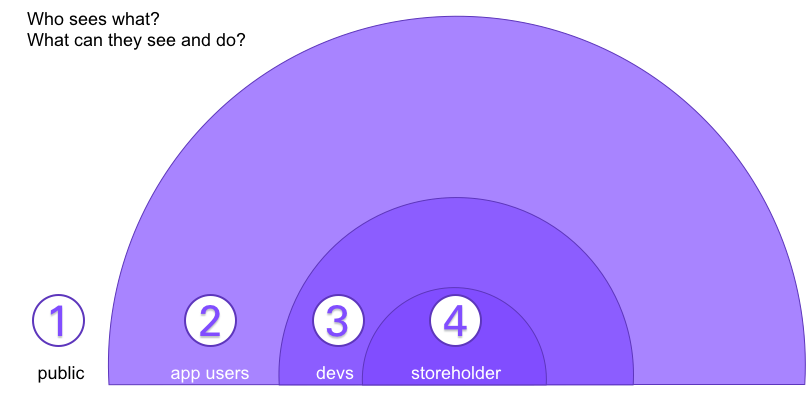
\includegraphics[width=12cm]{images/who-sees-what.png}
    \caption{Four Views of an App Store}
    \label{fig:4-views-of-apps-in-app-store}
\end{figure}

Figure~\ref{fig:4-views-of-apps-in-app-store} illustrates the four views; broadly, those closer to the centre can also see what those in outer rings can see. As a wise supervisor commented: \emph{``It's a bit like standing at different elevations on a mountainside and looking out over the landscape - the higher you are, the more you can see"}.

The first view is the public view of the app store, what is visible to someone who is not actively engaged with the app store. Examples include people who are not logged into their account, search engines, researchers mining the app store for ratings and reviews, and so on. The public is able to see aggregate ratings and some recent reviews for specific apps. Older reviews are generally hidden from public view (which may limit some research and search engine insights).

The next view is that of a user of a particular app or set of apps. They may have installed some of the apps directly, they are likely to also have pre-installed apps on their device too. They have the ability to interact with the app store, for instance they can see, create, and update their ratings and reviews~\footnote{If supported by the app store, for instance Google Play does.}. They can also see the public view.

%\akb{In the sentence below, does '.. records about their interactions ...' refer to the interactions of the developer or the user?}
Developers have the next view, which includes information the app store records about the developer's interactions with the app store, and information the app store provides the developers directly (\emph{i.e.} generated by the app store and related entities), as well as feedback provided by users via the app store (\emph{e.g.} ratings and reviews). Developers can also see the public view, although they cannot see the entire view of their user-base. However they can see any rating and reviews provided by the users.

%\akb{Do we know why the qualified 'often' is needed in the next sentence? Is this a non-deterministic behaviour of app stores and hence a forewarning of some of the data quality issues in the analytics platforms?}
Authors and developers are the two end points of ratings and reviews. Authors create them and developers receive them and can choose to respond to them, at least in some app stores. %these conversations. 
Importantly, their primary communications goes via the app store, rather than being direct, and aspects of these communications are often public for a period. Authors and developers can see their individual ratings and reviews for much longer periods than presented in the public view. The app store can use the ratings to decide on the quality of the app and their assessment may affect various important facets of the app's existence in the app store. For instance, well rated apps may be promoted and poorly rated apps may be demoted in search results. As Google states~\emph{``Apps whose metrics are higher have greater promotability, which raises their ranking in Google Play Store searches."}~\citep{android_vitals_best_practices} Also, poorly rated apps are sometimes subject to additional scrutiny and delays in the release process, as illustrated in Figure~\ref{fig:pocketpaint-to-help-better-protect-users} when the overall rating for a release dropped sufficiently to trigger this change. % The communications and implications will be covered later in this section.

\begin{figure}[htbp!]
    \centering
    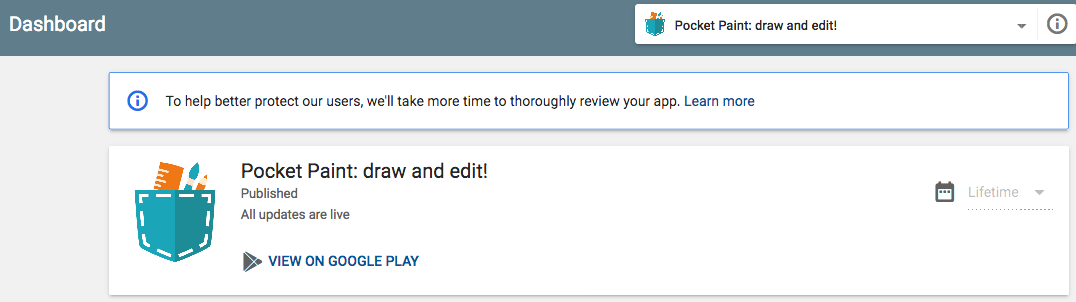
\includegraphics[width=15cm]{images/android-vitals-screenshots/pocketpaint-to-help-better-protect-users.png}
    \caption{Google Play message for Pocket Paint: To help better protect our users...}
    \label{fig:pocketpaint-to-help-better-protect-users}
\end{figure}

The final view is that of the app store, the `storeholder' in the figure. They have a global and holistic view of the entire store, including \textit{potentially}\footnote{A caveat on the use of potentially: this is because the app stores are closed systems with limited information about their actual behaviour in the public domain.} all the reviews, user interactions, and whatever usage activities have been performed by all the other three views. 
%\akb{Some explanation of the caveat term 'potential' here would be useful I think - i.e. this is because the app stores are closed systems with limited information about their behaviour in the public domain?}

We now cover various implications of the app store conceptual model.

\subsection{Trust relationships}
One of the key success factors of the modern app store (typified by the Apple App Store and Google Play) was that the platform provider provided the entire ecosystem and established the rules of engagement. The locus of trust is the provider of the app store, which acts as the public face and to some extent also acts as a representative for both the users and the developers. In terms of financial transactions it also acts as the intermediary and facilitates users being able to obtain refunds for app and in-app purchases subject to various conditions. 

Note: There are many details related to the trust relationships for those interested in that topic, however in the interests of focus and concision they are outside the scope of this thesis. 

\subsection{Communications paths and data flows}
There are numerous communication paths for mobile apps both with and without an app store being involved. As the vast majority of apps and users use devices and apps that are part of an app store ecosystem (even if they are obtained from other sources, e.g. as often occurs in India) I will only consider the ecosystem that includes an app store in this thesis. Figure~\ref{fig:sources-of-info-with-app-store-background-ch} illustrates various sources of information for apps available in an app store. The sources and communications paths will be considered next. 
% SHOULD-DO Perhaps a Venn diagram would also complement this illustration?

\begin{figure}[htbp!]
    \centering
    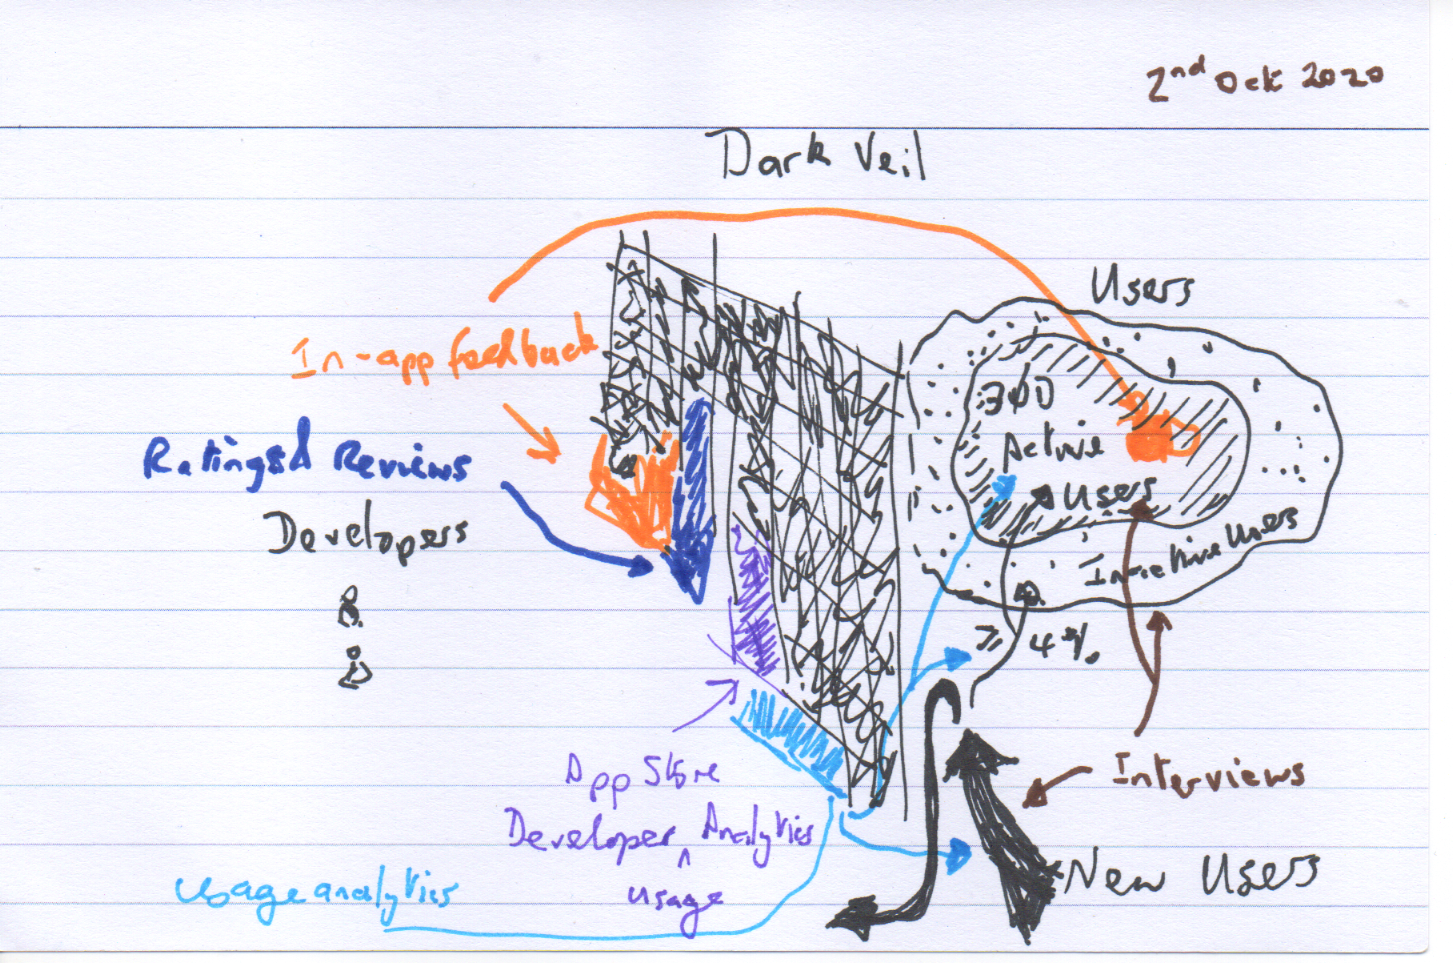
\includegraphics[width=13cm]{images/rough-sketches/sources-of-information-with-app-store-1.png}
    \caption{Sources of information with an App Store}
    \label{fig:sources-of-info-with-app-store-background-ch}
\end{figure}

The information about mobile apps can come from users directly or indirectly, from the app if it collects information either directly or indirectly, from devices. Such data collection could be via the operating system, installed apps with privileges to access information about other apps, from accessibility services, and potentially other means e.g. installed viruses. Alternatively, it could come from intermediaries - particularly the app store, and also from network traffic, observers,~\emph{etc.} 

Source code and source code repositories are also useful sources of information about mobile apps. Information can be usefully combined from several sources, for instance from source code about calls to write log messages compared to actual logs recorded when the app has been used on a device. Given the app store plays a pivotal role let's consider its role in terms of communication paths now. 

An app store is more than the store front, it controls and affects many aspects of the ecosystem that gathers around it. It is also more than the software, data and information that the various memberships can access. For instance the modern app stores often include software that is mandatory and pre-installed on end-user devices where that software cannot be easily removed or disabled by users\footnote{competent, technically savvy individuals may be able to thwart protection mechanisms as may other specialist organisations and software.} . This software includes a local storefront that offers end-users new apps, updates, and enables users to manage optional apps\footnote{Optional apps can be installed and uninstalled by end users at will. Non-optional apps are installed by various organisations, including the app store provider, some device manufacturers, and so on.}.

The app store provides various primary communications paths between the various parties involved in the ecosystem. It may be an active party, for instance in some of the reports provided to developers and/or users, and in policy-related matters; or it manages communications between app users and developers. Often the app store's owners define the rules of communications, including details such as whether and when apps can ask users to rate an app.

\begin{figure}[htbp!]
    \centering
    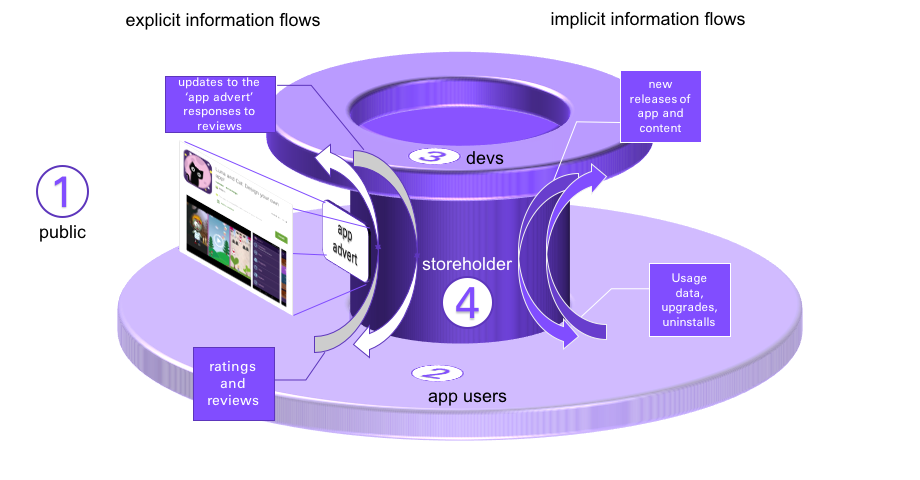
\includegraphics[width=17cm]{images/app-store-data-flows-3d.png}
    \caption{App Store: Communications Paths and Data Flows}
    \label{fig:app-store-data-flows}
\end{figure}

Some of the communications involves humans, or software chatbots masquerading as pseudo-humans intended to behave similarly to how humans would do in similar circumstances, for instance to provide in-app assistance~\citep{baez2020_chatbot_integrations} and to help developers respond automatically to app reviews~\citep{greenheld2018_automating_developers_responses_to_app_reviews}. Other communications is generated by software, for instance usage and diagnostic data collected by the operating system and related utilities on a mobile device (collectively described as the platform).

%\akb{Why are bots characterised as 'pseudo-humans'?}

The communications paths and data flows in an app store ecosystem are illustrated in Figure~\ref{fig:app-store-data-flows}. There are two forms of data flows: explicit and implicit. Explicit data flows are actively and intentionally performed by one or more of the participants, implicit data flows represents information that can be inferred or gleaned from various actions and inactions.

Examples of actions intended to communicate explicitly include:
\begin{itemize}
    \item Making the app available in the app store; this includes creating screenshots, a description of the app, adding meta data the app store requires and/or requests, \emph{etc.} This information becomes public if the app store approves the app for release.
    \item Ratings and reviews performed by app users. Only a subset of users provide these, the percentage varies from zero to a maximum of around 10\% with typical percentages around 1\% to 3\%. % SHOULD-DO find credible source for these estimates, I've checked various sources without success
    Estimates vary, partly as the definitions vary too. AppBrain states 46.5\% of Android apps do not have a rating~\footnote{Their definition is \emph{``Apps that have less than 3 ratings we consider to not have a rating yet"}~\url{https://www.appbrain.com/stats/android-app-ratings}}. In comparison, 42matters.com estimate 41\% of Android apps and 57\% of iOS apps have no rating~\footnote{\url{https://42matters.com/stats}}.
    \item Responses to reviews, for example Google Play allows developers to respond to reviews, and for both reviewers and developers to update their reviews and responses.
    \item Suspending an app so it is no longer available to users to download. Storeholders sometimes suspend apps and even developer accounts where they perceive the app and possibly the developer contravenes the app store's policy. % c.f. the recent ban of Fortnite in both Apple and Google stores. And see the comment after this article re German law https://www.overpass.co.uk/google-play-account-suspended/ 
    %\href{https://www.ape-apps.com/viewpage.php?p=34186}{My Colony Suspended from Google Play}
    %\href{https://www.ape-apps.com/viewpage.php?p=34173}{My Colony removed from Google Playstore} - over 50% of users come from Google Play.
    
\end{itemize}
%%%%%%% Various interesting sources of Android- (and some iOS) related stats
% https://www.businessofapps.com/data/app-statistics/
% https://www.statista.com/statistics/266217/customer-ratings-of-android-applications/ (seems to be a rehash of AppBrain's report)
% https://mindsea.com/app-stats/
% 

%\akb{Use consistent labels for concepts - below you refer to '(implicit) information flows' whereas above you use '(explicit) actions intended to communicate'.  By using different labels you are suggesting that these two implicit/explicit categories are not directly comparable, i.e., they are different types of things altogether. However, I am not sure this is your intent.}

Implicit information flows include:
\begin{itemize}
    \item New releases of apps and related content (such as in-app content, often purchased using in-app purchasing). These indicate the developer is wishes to actively engage their userbase. Upgrades may include changes to the app seeded by various sources such as ratings and reviews and other data, including:
    \item Usage data and upgrades, both imply the software provides some value to the users. Lack of usage may also be an indication the software is not currently providing value - this may be expected for instance with seasonal apps. Uninstalls are a stronger signal that users no longer see sufficient value in the app to keep it on their device.
\end{itemize}

On-device bug reports may be a hybrid, where the bug reporting utility on the device does much of the data collection and may report this automatically and transparently, however it may sometimes ask the user for additional input and permission to send the bug report.

\subsection{Membership criteria of each group}
%\akb{Explain why the membership criteria are important to understand, perhaps combine with next section single explanation of groups and what members can do in each}
As Figure~\ref{fig:app-store-data-flows} illustrates there are four numbered groups in the illustration. People can potentially belong to more than one group (albeit membership of the storeholders is limited to owners and those they assign membership to,~\emph{e.g.} as administrators of the app store). Group membership constrains what the members can do as participants and what they have access to.

\begin{enumerate}
    \item Public: the membership criteria are minimal. Here `public' is any entity, human or technological, that has access to the app store\footnote{For our purposes we can assume online digital access, other modes may also be viable, for instance some researchers use archives of data sourced from app stores.}. An example of a technological entity, is a search engine crawler or software including web scraper technology and scripts that use APIs provided to obtain information about apps in the app store.
    %\akb{Not sure what is meant by 'minimal' here. You could describe 'public' as any entity, human or technological, that has access to the app store. Provide an example of a technological entity, e.g., a search engine crawler}
    \item App user: the public can use an existing account or create a new account with the app store that would allow them to become an app user~\footnote{They need to meet the criteria of the app store.}. Note: there may be restrictions or constraints that mean not everyone can install every app on every device, however the general practice is that apps are freely available for app store users to install on any device they possess. 
    \item Developer: developers need to be registered and validated by the app store, the process varies for specific app stores, they often involve payment of a fee and some amount of validating their identity. Some app stores may perform additional checks based on information they and/or others hold.  
    \item Storeholder: they are generally a legal entity, and certainly for the purposes of this research they are. Apart from a few exceptions (such as F-Droid~\footnote{Details are available online at~\url{https://www.f-droid.org/en/about/}}) they are multi-national major corporations.
\end{enumerate}


\subsection{What participants can and cannot do (and who dictates the rules?)}
%\akb{You don't explain the link between the implicit/explicit data flows and these membership groups.}
\begin{itemize}
    \item Public: The public cannot review an app or easily download the app. They can view publicly accessible information, including information that was gathered previously, potentially by others.
    \item App user: They can rate and review apps they have installed on their account~\footnote{ user may have several devices and choose not to install an app on all of them. Also some apps may by limited to devices that meet particular criteria e.g. the platform version.} or device. They can also install, update and deinstall apps~\footnote{There may be restrictions imposed for some apps, for instance Google Apps and Manufacturer apps might be blocked from being uninstalled, and updates are sometimes mandatory, \emph{etc.}}.
    \item Developer:  Approved developers can upload apps to the app store and publish them if the app store also approves the release. They can choose to submit new versions of their apps, sometimes they may be required to do so by the app store. They can choose to suspend or withdraw their app from the store, note: generally users can continue to use the app if they have it installed. Developers are expected to interact with the app store and often do so of their own volition, for instance to see how their app is `doing'. The developer may define a price for their app and/or any in-app purchases. They may also require users comply with additional terms of use, and many apps do so.
    \item Storeholder: They are by far the most powerful participant as they establish the ecosystem including the rules of engagement and enforce these rules. The app store has the right of delay or veto of releases, it can suspend apps and developers, and much else besides. They are expected to comply with the laws of the various countries the app store is available in and also where their business is situated. These laws may affect the developers and the app users, for instance the amount of sales tax charged on a purchase in the app store.
\end{itemize}

We have already identified four membership groups involved in app store ecosystems, there is at least one more and also additional data flows in the ecosystem. The fifth membership group is a~\emph{service provider}. These service providers provide non-trivial functionality and other capabilities such as in-app analytics, feedback, and so on. Developers can choose to incorporate software libraries into their apps and use the services provided, for instance as conduits of communications between the app and the developers. Here developers include other specialist groups in their organisation such as customer service personnel and marketing teams. Many app developers choose to use at least one such service, some incorporate several and there is even specialist software that enables developers to manage multiple similar services within their apps on end-user devices. An example of this type of software is~\url{https://github.com/segmentio/analytics-android} (other platforms are also supported and there are other providers of similar software).

Membership matters in particular because of who has access to which data and for how long they have access. Note: Control and `ownership' of the data are also relevant topics, however they are not necessary to comprehend the rest of this topic. % SHOULD-DO consider whether to add material on this topic in the thesis. 

\section{Conceptual model of layers within apps and observation points}
Observation can be internal,~\emph{i.e.} built into apps, and external. External includes instrumentation, debugging tools, the operating system at runtime, accessibility interfaces, event listeners, log watchers, and so on (as this is not intended to be an exhaustive list). The observation may also be indirect, for instance using network monitoring software, and/or from remote APIs, REST endpoints, and web servers (with their attendant logging).

\subsection{Three layers of an app}
In earlier work, published in ~\citep{harty_aymer_playbook_2016}, the concept of three layers of an app was introduced. These are illustrated in Figure \ref{fig:3-layers} and shows three primary conceptual layers related to a mobile app. 

\begin{figure}[htbp!]
    \begin{minipage}{\textwidth}
    \centering
    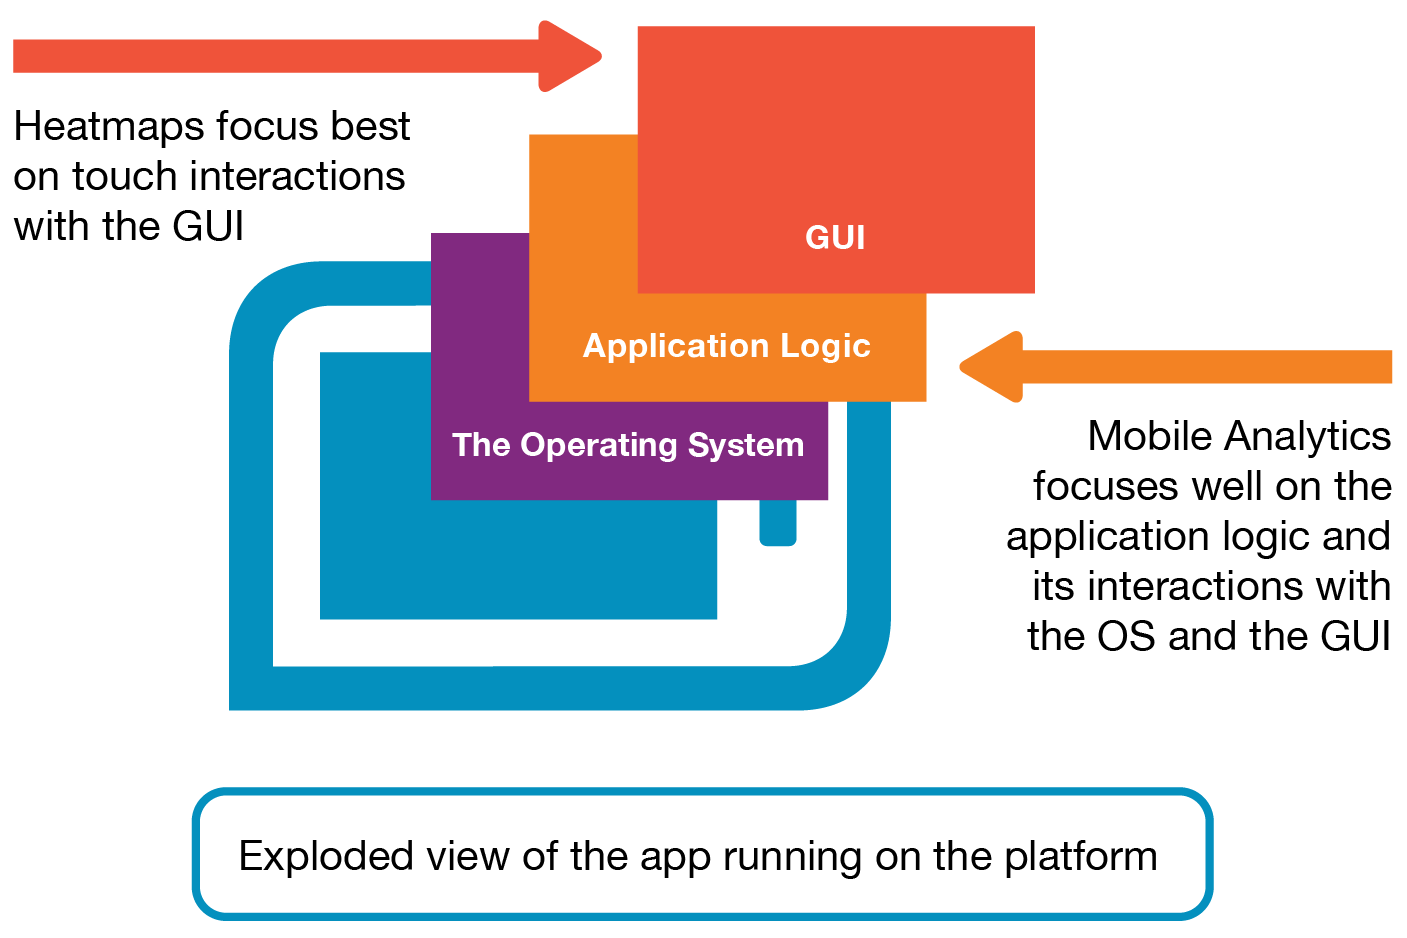
\includegraphics[width=10cm]{images/mobile-analytics-playbook/3-layers.png}
    \caption[Three layers of an app]{Three layers of an app~\footnote{Image credit: First published in The Mobile Analytics Playbook~\citep{harty_aymer_playbook_2016}}.}
    \label{fig:3-layers}
    \end{minipage}
\end{figure}

Of course, apps aren't quite this simple or well defined in reality, for instance they include software libraries from various sources, A/B testing utilities, logging code, run-time lifecycle management, and so on. Nonetheless, these three layers are a useful abstract, particularly in terms of useful observation points about apps on user's computer devices~\footnote{Another observation point that was orthogonal to the application logic layer was one popularised by a company that has since been acquired, called SafeDK. They provided app developers with software that provided an interface between the developer's code and the libraries the code used. This software collected and reported usage data on the performance and reliability of the libraries. Given the commercial nature of the business, their acquisition and the demise of their products and the company's website, and the fast moving nature of the internet, obtaining concrete information may be impractical for all but a few people who know those who were involved at the time.}.

The Graphical User Interface (GUI) % SHOULD-DO add to glossary.
can be visually observed by sighted users, it can also be observed by Accessibility software, and test automation tools, \emph{etc.} externally to the app. It can also be observed from within the app, for instance through using software known as \emph{heatmapping} that records the screens and the touch interactions performed by users of that screen. One of the the more popular, mature heatmapping offerings is from AppSee~\footnote{\url{  https://www.appbrain.com/stats/libraries/details/appsee/appsee}. Note: in 2019 Appsee's team was acqui-hired by ServiceNow~\url{https://techcrunch.com/2019/05/13/servicenow-acquihires-mobile-analytics-startup-appsee/} and the service no longer directly available.}, nonetheless they are only used in a small minority of mobile apps.


\subsection{Observation points: inside-outside perspectives}
The observation point determines what can be observed and how. 
As Figure~\ref{fig:internal-external-table} illustrates there are internal and external perspectives on an app for various purposes, including observations, interactions (e.g. through test automation), and emitting information (e.g. through logging, reporting, or mobile analytics). Where the information is observed affects what can be known and what is possible, an insider is privy to information an outsider is not; whereas an outsider has perspective and can potentially perceive things insiders cannot.

\begin{figure}[htbp!]
    \centering
    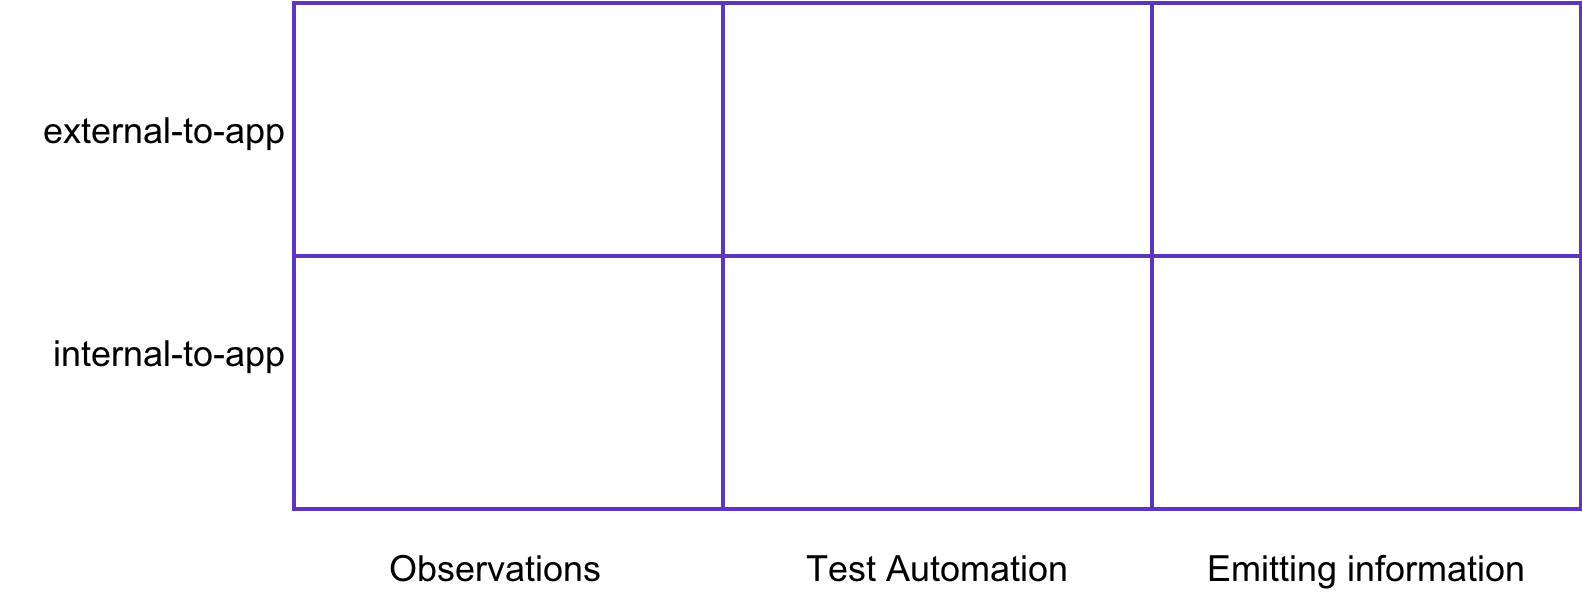
\includegraphics[width=13cm]{images/internal-external-table.png}
    \caption{Internal and external perspectives of an app}
    \label{fig:internal-external-table}
\end{figure}

%\textbf{SHOULD-DO} Expand the following: What is test automation? discuss how mobile apps are tested, the unique aspects of using accessibility interfaces, etc.

\section{Conceptual model of analogue and digital feedback}~\label{analogue-and-digital-feedback}
Feedback can help developers to find and choose ways to improve their software. Various researchers have investigated way to understand and use feedback provided by end-users, for instance, in ratings and reviews users provide to the app store. For the purposes of this research feedback people provides is considered~\emph{analogue feedback} as it has the richness and complexity of analogue signals, and also challenges of processing and comprehension.

In contrast, digital feedback originates from software and is generally deterministic~\footnote{~\url{https://en.wiktionary.org/wiki/deterministic}}. For the purposes of this research~\emph{digital feedback} is provided by running software where programmers added code to programs to collect data that provides feedback about software use and certain behaviours of that software. The addition of the code may be automated, in part, or wholly, for instance by another program or script. As an example, AppPulse Mobile claims they can add analytics automatically without developers writing a line of code~\footnote{~\url{https://www.microfocus.com/en-us/products/apppulse-mobile-app-apm-monitoring/overview}}.

\begin{figure}[htbp!]
    \centering
    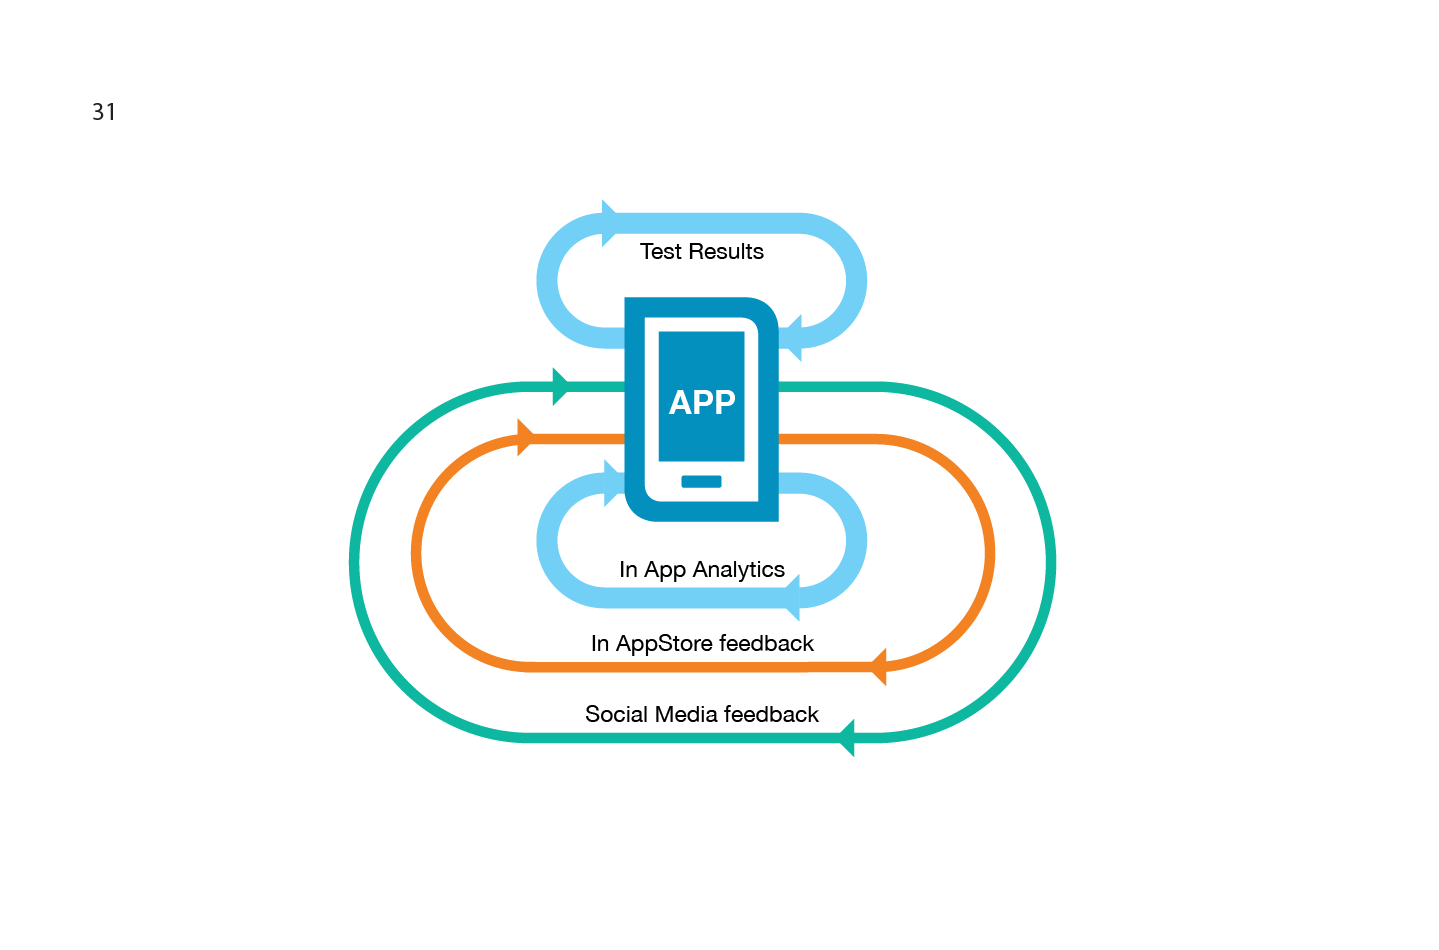
\includegraphics[width=15cm]{images/mobile-analytics-playbook/Chart-07-FeedbackLoops.png}
    \caption{Feedback Loops for mobile apps~\citep{harty_aymer_playbook_2016}}
    \label{fig:map2015-feedback-loops-for-mobile-apps}
\end{figure}
%SHOULD-DO edit the figure to remove whitespace, etc.

Figure~\ref{fig:map2015-feedback-loops-for-mobile-apps} illustrates various feedback loops where the feedback could be used to change and improve a mobile app. Within the team's aegis are test results (and static analysis, etc.). Beyond their direct control are feedback within the app, within the app store, and outside the app store ecosystem such as feedback on social media about their app. This figure illustrates in-app analytics which was the primary form of analytics at the time the figure was published, since then two additional forms of feedback have emerged: platform-level feedback such as Android Vitals and in-app feedback.

\subsection{Analogue feedback: in-app tools}
One source of feedback is when apps include feedback mechanisms within the app. Various benefits are touted to encourage developers to add such feedback including the ability to: ~\emph{``...capture valuable insights into the usability of the app and quickly resolve any issues..."}~\citep{mopinion2017_top11_mobile_in_app_feedback_tools}, for example. 

Some apps also collect in-app feedback if the user indicates they are not satisfied with the app and conversely ask users to submit a review online in the app store if they are satisfied. One hypothesis is their developers have implemented this approach to divert adverse ratings and reviews from public view and from the app store algorithms. 

In-app feedback enables a wider range of communications and also scope for richer dialogues than relying on feedback mechanisms provided by app stores which consist of a rating and an optional plain text comment. Examples of wider ranges of communications include surveys, and richer dialogues include audio recordings.

In-app feedback has also been proposed for bi-directional communications between developers and users of the app for instance to elicit non-functional requirements~\citep{avellis_harty_yu_towards_mobile_twin_peaks}.

\subsection{Analogue feedback: app store feedback}
App store feedback, combines a rating (typically using a one- to five- start rating and an optional plain-text comment). It is a subject covered by significant volumes of research and discussed in the related works chapter. %MUST-DO actually write up this related research and contrast it with mobile analytics.

\begin{figure}[!htbp]
    \centering
    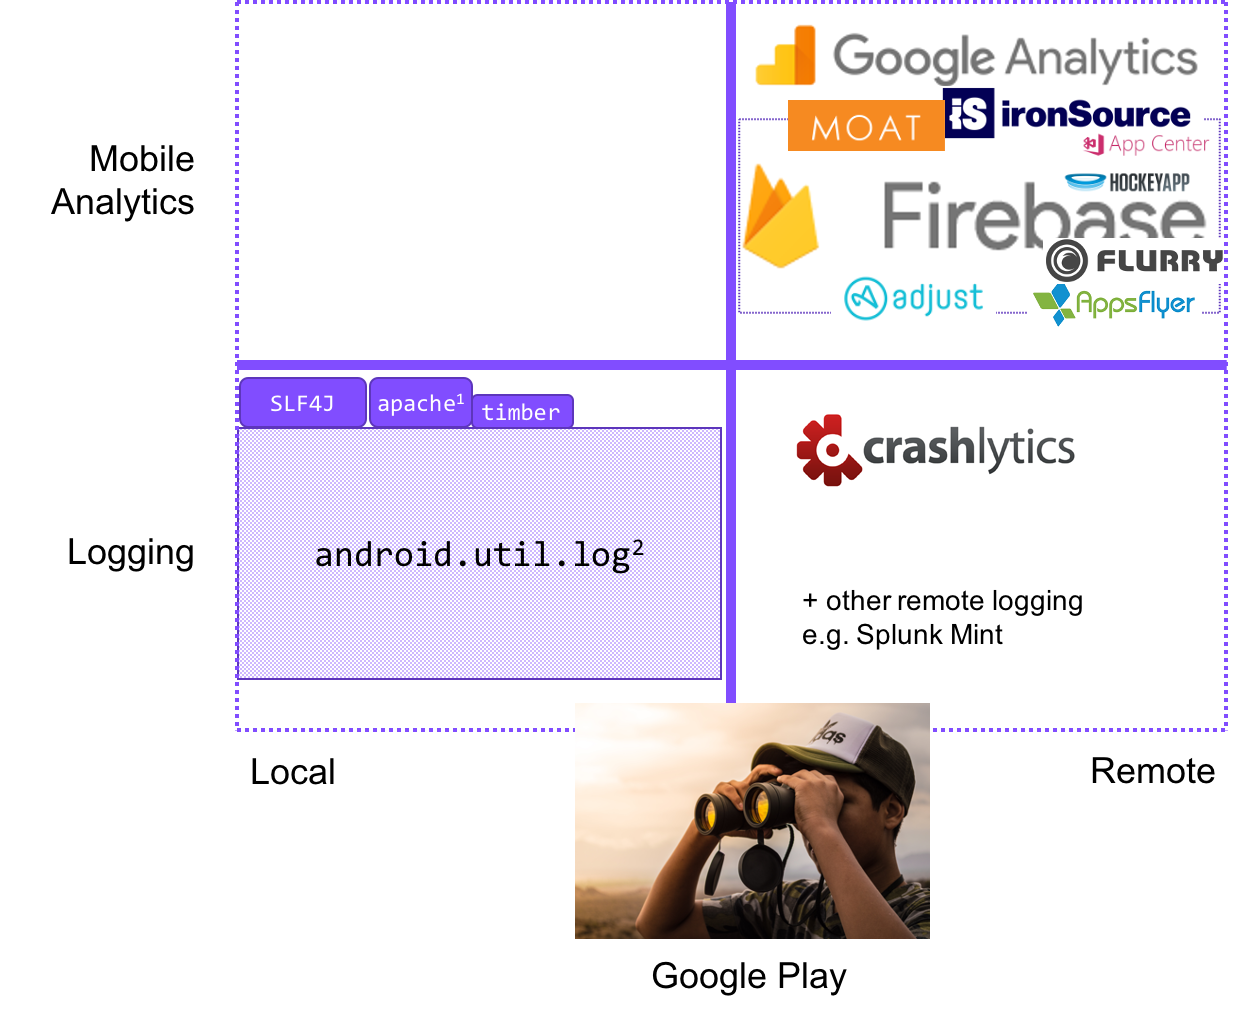
\includegraphics[width=12cm]{images/matrix-of-logging.png}
    \caption{Matrix of logging}
    \label{fig:matrix-of-logging}
\end{figure}

\subsection{Digital feedback: logging and mobile analytics}
The application may incorporate logging and/or mobile analytics. Logging in mobile apps is often used locally, by developers independently of other mechanisms. Mobile analytics is used remotely, as are crash reporting libraries. 



Figure \ref{fig:matrix-of-logging} illustrates a matrix of logging, where logging and mobile analytics are on the Y axis and local and remote on the X axis. There is a cross-cutting example where the mobile platform observes local events and then forwards the information remotely. A good example is Google Play which appears to be an external observer of data recorded in device logs. Data collection runs locally and is sent to Google servers where Google analyses the data and provides reports to developers for their apps. %SHOULD-DO check for related US patent filings by Google in this area.

\begin{table}[!htbp]
    \centering
    \begin{tabular}{lll}
         Category of logging &Local access?  &Remote access? \\
         \hline
         None            &N/A  &N/A \\
         \texttt{StdOut} &It depends &Unlikely \\
         Default platform logging library &Yes &Possible \\
         Enhanced platform logging library &Yes &Possible \\
         Third-party logging library &as-designed &as-designed \\
         Proprietary logging library &as-designed &as-designed \\
         
    \end{tabular}
    \caption{Choices available to developers for logging in mobile apps}
    \label{tab:logging-choices-for-devs}
\end{table}

Table~\ref{tab:logging-choices-for-devs} identifies various categories of logging available to developers of mobile apps. They range from no active logging in the app (some information is still logged by the platform) to proprietary custom logging libraries which a tiny minority of development teams would chose to do - they may do so to keep their logging as private as practical from the rest of the device.

\texttt{StdOut} is often used in code written for other platforms including Linux that has been ported to mobile platforms. Some people who are unfamiliar with logging libraries who have a superficial understanding of developing for mobile devices may also use print statements in their code (which effectively writes to the standard output) rather than use log statements in their code. There are various nuances of how the standard output and standard error outputs are handled in Android code (Java, Kotlin, etc.) and native code (C/C++) are directed as standard for Android apps. In short, for native code (\emph{e.g.} written in C/C++) as standard the outputs are discarded by `writing' them to~\texttt{/dev/null}. For Android code (\emph{e.g.} written in Java/Kotlin) \texttt{System.out} and \texttt{System.err} can be redirected to the log on some Android releases if the device is configured to do so.
%MUST-DO add references for https://github.com/android/ndk/issues/671 and https://codelab.wordpress.com/2014/11/03/how-to-use-standard-output-streams-for-logging-in-android-apps/ and https://stackoverflow.com/a/17199704/340175 and https://stackoverflow.com/questions/10531050/redirect-stdout-to-logcat-in-android-ndk

There are various enhanced log libraries, for instance~\texttt{timber} which are used by discerning app developers. These libraries also write to the platform log files. 

To Be Continued. %MUST-DO

\begin{figure}[htbp!]
    \centering
    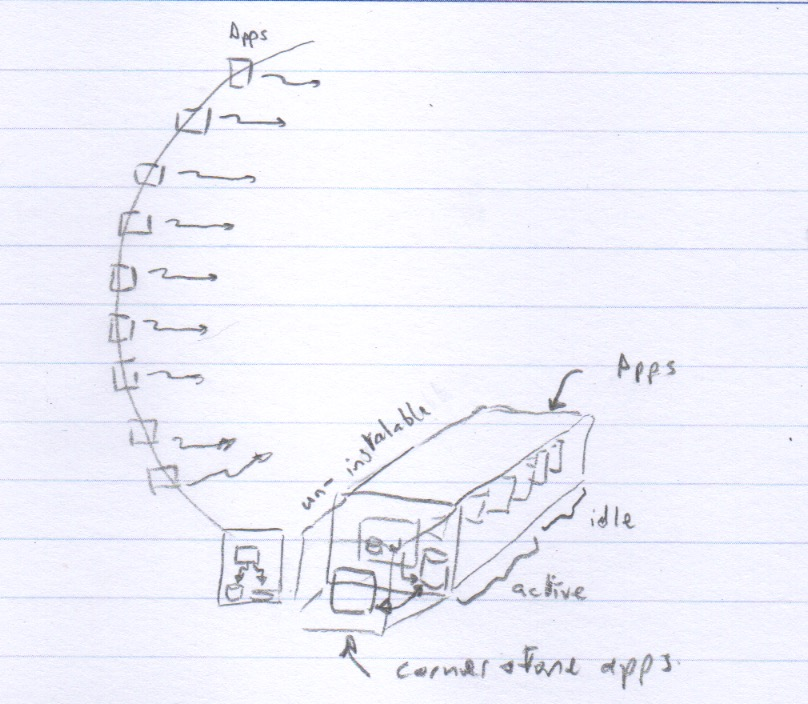
\includegraphics[width=12cm]{images/rough-sketches/apps-on-device-boundaries-sketch.jpeg}
    \caption{Apps on the device boundaries}
    \label{fig:apps-on-device-boundaries}
\end{figure}

\begin{figure}[htbp!]
    \centering
    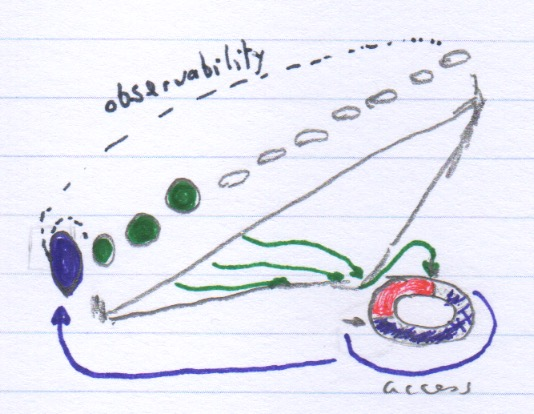
\includegraphics[width=8cm]{images/rough-sketches/on-device-logging-sketch.jpeg}
    \caption{On-device logging}
    \label{fig:on-device-logging}
\end{figure}

A couple of rough sketches, Figures~\ref{fig:apps-on-device-boundaries} and~\ref{fig:on-device-logging} present two views of apps installed on any given mobile device. These apps are broadly one of three categories: platform, pre-installed (non-removable), and user-installed (removable). Here the focus is on their use of logs on the device.

At any point one or more of these apps may be running, the rest are idle. The majority of these apps, with the possible exception of system apps, write to one or more shared, common, log files. These log files have a finite size, and once they are filled newer messages overwrite the oldest ones in turn. In Figure~\ref{fig:on-device-logging} the left-most blob, in purple, represents a system app that is able to read the shared system log files. These apps are pre-installed by the manufacturer, they may include those from the provider of the platform, particularly from Google for Android devices that use Google Play, and also some device manufacturers may have similar apps. Other apps are also pre-installed by manufacturers including a suite of apps from Google and some from the manufacturer. They may also include apps from organisations with agreements with the device manufacturer, for instance they may pre-install some games and utilities from partners. TBC.


As an observation the vast majority of Android developers use the default inbuilt logging library \texttt{android.util.log} and choose one or more of Google's analytics offerings (which include Firebase and Crashlytics). A commercial organisation, AppBrain, provides current statistics for third-party logging libraries~\footnote{Logging libraries (note the default android log library is not tracked at the time of writing~\url{https://www.appbrain.com/stats/libraries/tag/logging/logging-libraries}}, crash libraries~\footnote{\url{https://www.appbrain.com/stats/libraries/tag/crash-reporting/android-crash-reporting-libraries}} and mobile analytics~\footnote{\url{https://www.appbrain.com/stats/libraries/tag/analytics/android-analytics-libraries}}. Some apps have several of these libraries so counts may exceed 100\% in their reports.

\begin{itemize}
    \item Logging: enables developers to understand what their software is doing. The practice is commonplace across many software domains including mobile apps, and each platform and language includes a standard method of generating log messages. These messages tend to be small and intended for immediate, local consumption. On Android when developers use the standard logging library (\texttt{android.util.log}) their log messages are written to a shared circular log file on a device. As illustrated in Figures~\ref{fig:apps-on-device-boundaries} and~\ref{fig:on-device-logging}, some privileged Android software is able to read these shared logs. Developers can also read them using standard Android development tools \emph{e.g.} \texttt{adb logcat} providing they are connected to the device with the log file. Older versions of Android allowed apps to read the full contents, more recently apps are restricted to only the log messages they wrote unless they are granted the relevant permission by Google and the user. 
    In other domains \emph{e.g.} web servers, infrastructure software, and many others, logging is used for production monitoring, fault-finding and analysis. A minority of mobile app developers use remote logging.
    \item Mobile analytics, can extend and scale logging. For mobile analytics, a minority of developers incorporate custom implementations, however the vast majority who use analytics do so through using third-party analytics libraries such as Google Firebase Analytics, details of the current usage of analytics libraries are provided by AppBrain~\footnote{\url{https://www.appbrain.com/stats/libraries/tag/analytics/android-analytics-libraries}}.
\end{itemize}

One of the appendices, ~\href{chapter-on-mobile-analytics}{\textit{on mobile analytics}}, provides details of the design of content and messages together with the mechanics of sending the data; in terms of establishing a grounding in this topic it is enough to be aware that these are both relevant aspects of incorporating and using mobile analytics.


\begin{figure}[htbp!]
    \centering
    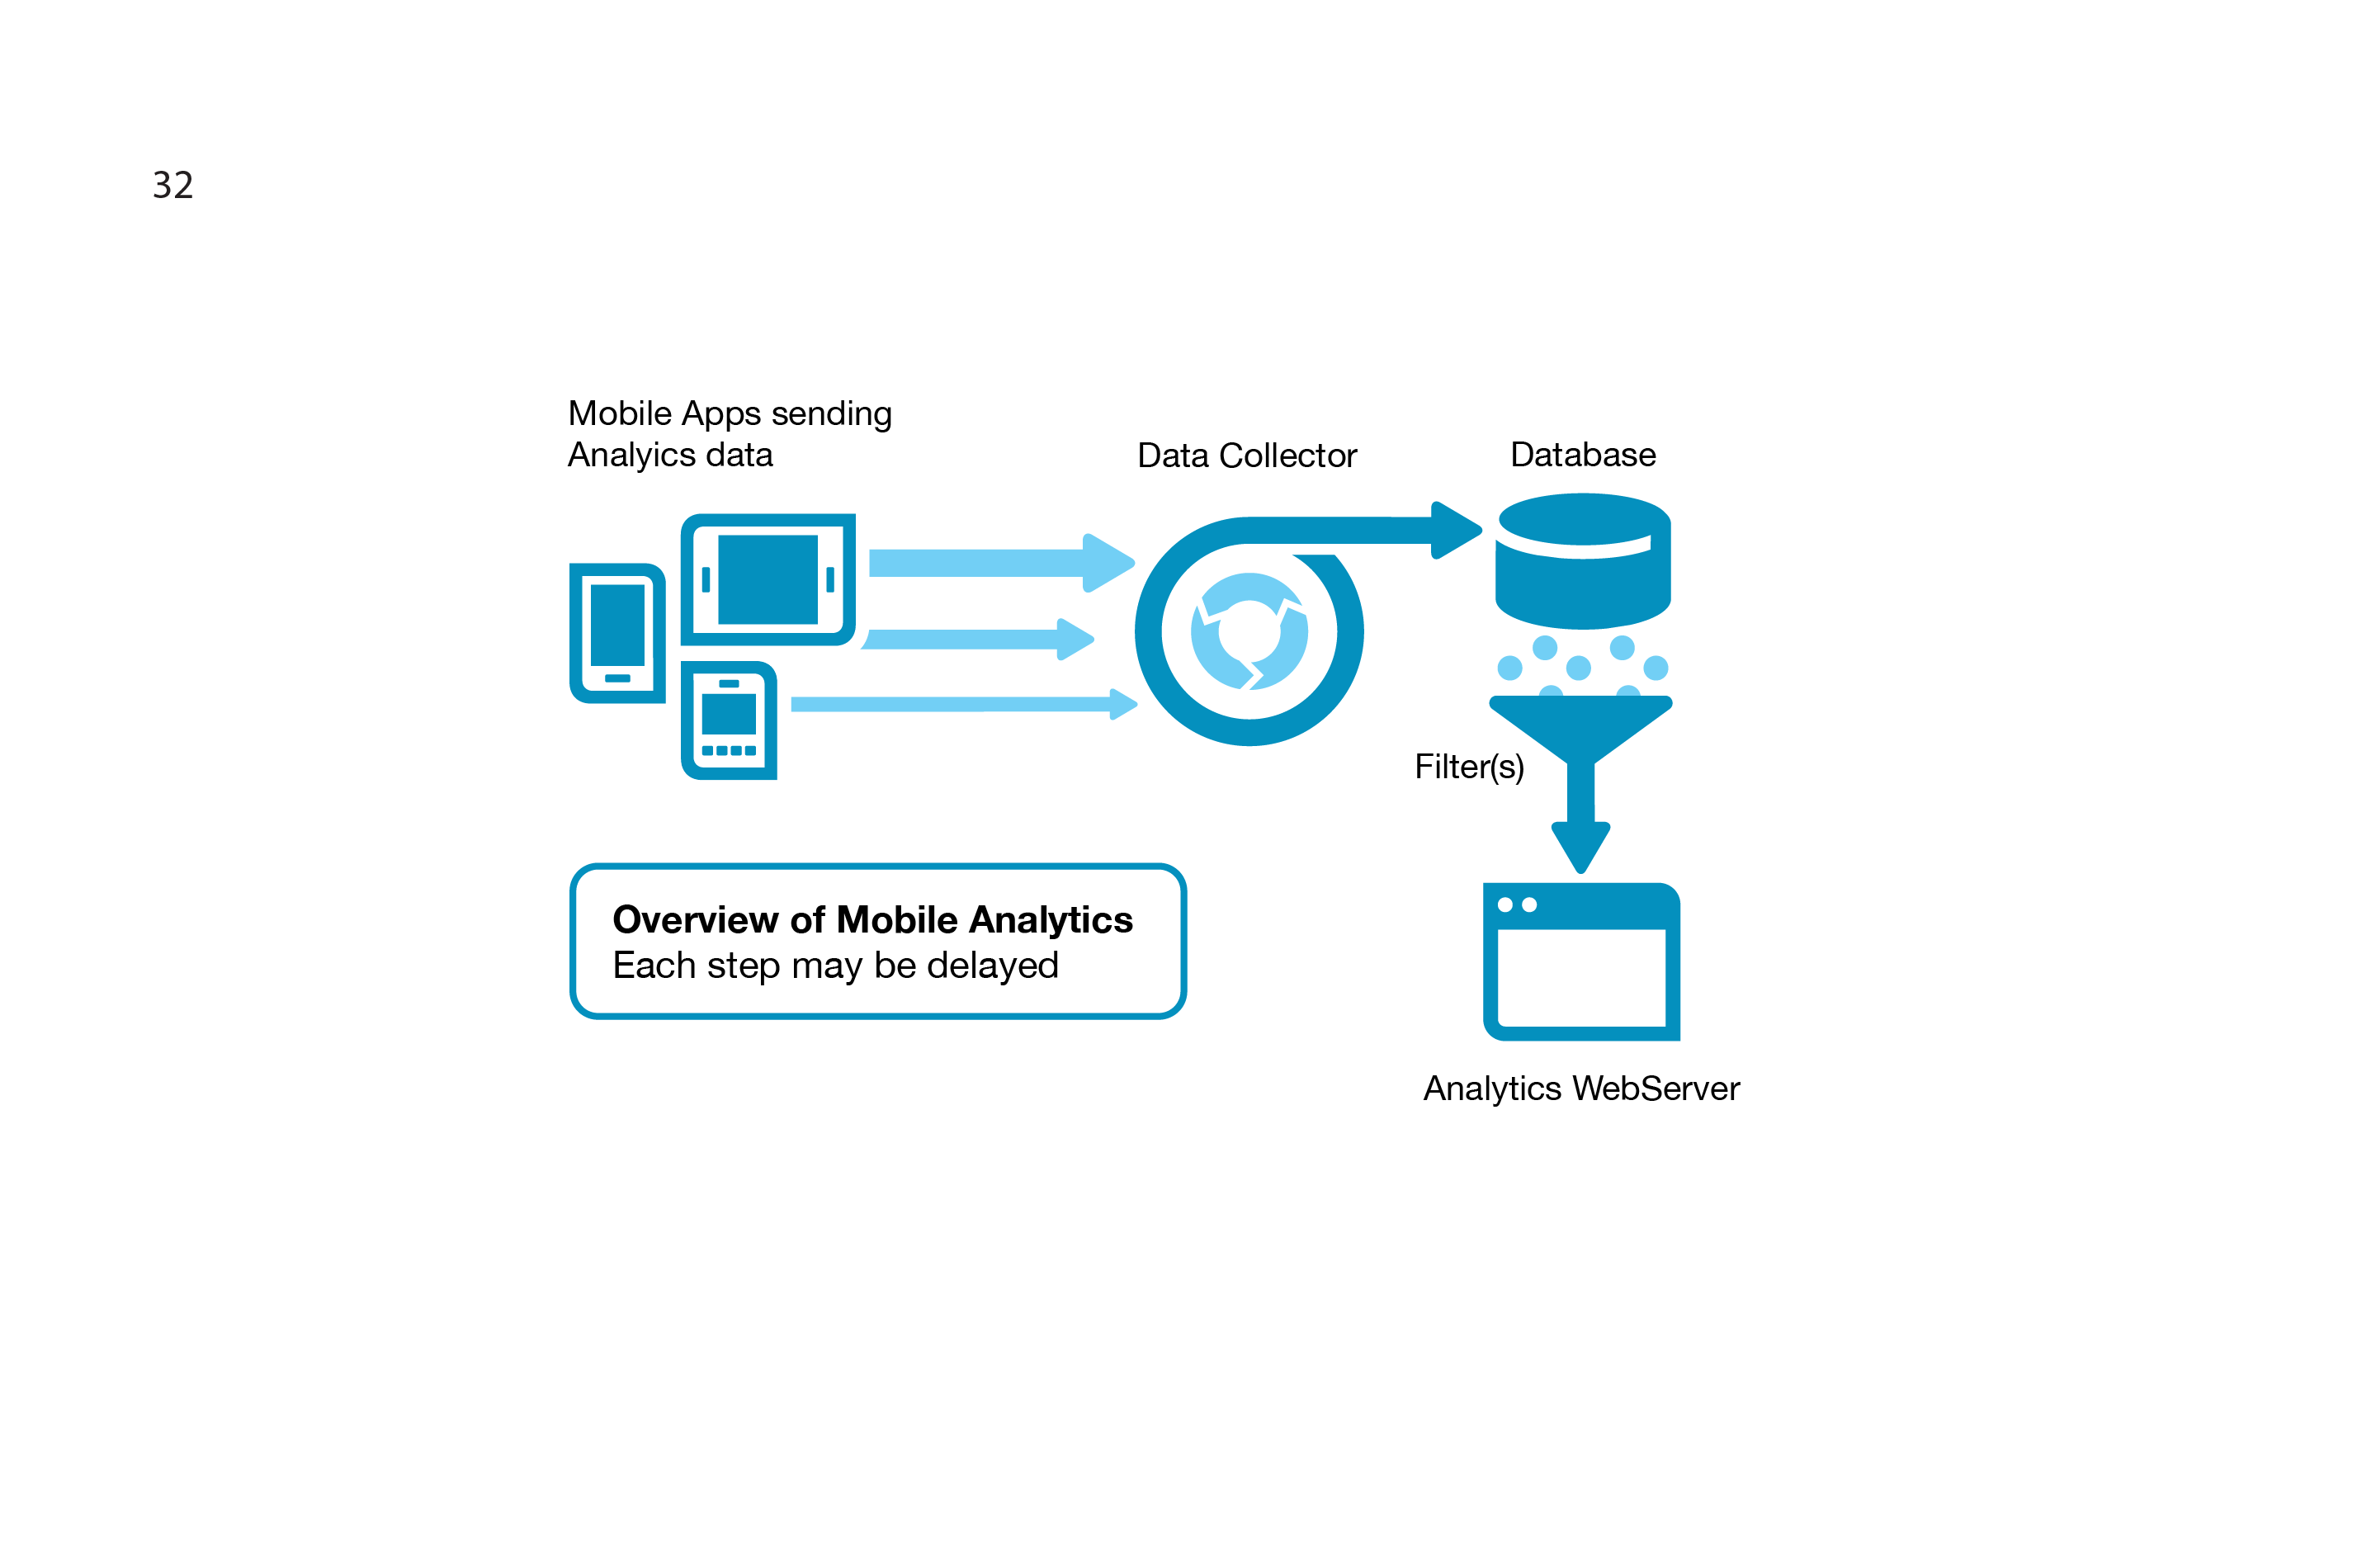
\includegraphics[width=15cm]{images/mobile-analytics-playbook/Chart-08-Overview-of-MobileAnalytics.png}
    \caption{Overview of Mobile Analytics~\citep{harty_aymer_playbook_2016}}
    \label{fig:map2016-overview-of-mobile-analytics}
\end{figure}

An overview of Mobile Analytics was published in The Mobile Analytics Playbook,~\citep{harty_aymer_playbook_2016}, and the figure is reproduced here with permission in Figure~\ref{fig:map2016-overview-of-mobile-analytics}. The overall approach also applies conceptually in terms of how either apps (often delegated to the analytics library implementation) or the device sends the data. As an observation, the approach would also work if the data is transferred using other conduits, such as copying the data using a memory card, however these details are unlikely to apply to the vast majority apps and even for those developers the conceptual model is unlikely to change materially.

Transmission of the contents of the logs and/or mobile analytics data is asynchronous and may occur almost immediately, or in some rare cases months later. In a discussion on the Android implementation of the popular segment.io library, a non-profit reading app needs to store up to six months of reading analytics on the device using this library. The authors discussed practical ways to store the analytics events without loss and then to be able to upload them correctly even where network connectivity is unreliable~\citep{segmentio_supporting_6_months_offline}. Several analytics providers have documented their transmission mechanisms. \emph{``Crashlytics limits logs to 64kB and deletes older log entries when a session's logs go over that limit."} and it~\emph{``...only stores the most recent eight recorded exceptions. If your app throws more than eight exceptions, older exceptions are lost."}.  The non-fatal exceptions are sent the next time the app launches~\citep{firebasecrashlytics2020_customize_crash_reports}. In contrast the Segment implementation for Android stores up to 1000 events~\citep{segment_analytics_for_android_docs}.

One of the particular implementation details may be worth considering, which is the growth in intermediaries and their adoption by developers. Segment provides one such service, where they provide developers with a single per-client app API that then wraps hundreds of potential implementations and offers two \emph{``connection modes"}, device and cloud~\citep{segment_analytics_for_android_docs}. When using their cloud-mode~\emph{``Segment sends messages to the Segment servers, and then translates and forwards that data on to the downstream tools."} Their service becomes a vital additional component in the process and may affect many aspects of the data including privacy, who can analyse it, and latency implications.   

\subsection{Data funnels from users to devs}
The following list itemises a set of possible stages in a data funnel for data that originates from a user's device until it is available for use by the development team. real-world funnels are likely to include a subset of these, in a particular order in terms of the data flow.

\begin{itemize}
    \item Per-app implementation and options
    \item Per-analytics/logging library implementation and options
    \item Farming the log (and/or potentially other usage data) data on device
    \item Device model and operating system combination
    \item Per device implementation and options
    \item Data daemons that control/negotiate what data is and is not available/provided
    \item Data privacy screening (can occur at various points in the funnel)
    \item Batching, queuing, limits, latencies, transmission triggers, ...
    \item Connectivity quality and reliability
    \item Network behaviours e.g. where traffic may be blocked in some geographies, by some network providers, etc.
    \item Data Collector inbound processing (filtering, buffering, validity checks, non-repudiation, dealing with spoofing, fakes, etc.)
    \item Analytics tool filtering and reporting. This may include muting of some aspects of the reporting e.g. for issues considered no longer actionable. 
    \item Content access, storage, combination with other sources, further reporting, etc.
\end{itemize}

Note: there may also be data injected into the funnel, for instance through \href{https://en.wikipedia.org/wiki/Synthetic_monitoring}{synthetic monitoring}, testing of the apps and/or the analytics clients and APIs, spoofing, denials of service, and so on. 

MUST-DO add figure, write up this section.




\section{Conceptual model of usage analytics}
Usage analytics pertains to recording and analysing the usage of software. Application usage analytics is mentioned in various sources, including patents filed by Google in the USA~\emph{e.g.} for methods and systems to collect and provide application usage analytics to developers~\citep{googlepatent_hyman2016_collecting_application_usage_analytics}. 

Conceptually there appear to be four broad levels of usage analytics, these are illustrated in Figure \ref{fig:four-layers-of-analytics-for-mobile-apps} and described next. These four levels can be approximately mapped~\footnote{The approximation is because software is not quite so cleanly cut into layers or levels. For instance app-level mobile analytics can be used to record many aspects of GUI activities, albeit unnaturally. Also, the operating system can observe aspects of the GUI, for instance by instrumenting the Accessibility APIs, a topic I touch on in one of the appendices.} to the three layers of an app:

%\akb{Are 'Visual' analytics tools automatically 'Mobile' tools as well? The \textit{heatmapping} example seems to be one that could fit into both layers}

Their use will be discussed in more detail in the chapter titled~\href{chapter-applying-analytics-to-development-practices}{\emph{\nameref{chapter-applying-analytics-to-development-practices}}}. %MUST-DO decide whether layer and level are synonymous, and if not whether to use one term or the other. Anyway I'm aware I may be conflating both terms here and want to improve the precision of whichever term(s) I use. 

\begin{figure}[htbp!]
    \centering
    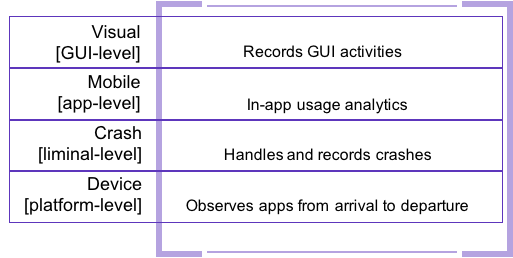
\includegraphics[width=12cm]{images/4-layers-of-analytics.png}
    \caption{Four Layers of Analytics for Mobile Apps}
    \label{fig:four-layers-of-analytics-for-mobile-apps}
\end{figure}

\begin{itemize}
    \item \textbf{Visual (GUI-level)} operates at the GUI level, or layer, of the app. It records aspects of the GUI activities such as touches, gestures, interactions with the screen, and data entry. Often it includes recording what is on the screen too. A common type of Visual analytics is \emph{heatmapping} software. Note: visual analytics may be \emph{implemented} in the app, conceptually they observe the GUI as if from above the UI.
    \item \textbf{Mobile (app-level)} is incorporated as part of the app and records aspects of what the app is doing, in effect aspects of the usage of the app. Mobile Analytics is prevalent in Android apps and already used for various business purposes.
    \item \textbf{Crash (liminal-level)} is where specialised reporting can intercept crashes. Through the interception they can change the behaviour of the app, for instance to provide a better user-experience, log, and report the crash to the developers. \emph{Fatal crashes} are ones where the application quits. These can also be observed by the operating system; for mobile apps the operating system is an intrinsic part of the platform.
    \item \textbf{Device (platform-level)} Platform-level analytics can record apps from when they are installed until they are removed. This recording can include details such as when apps are in-use, crashes, freezes, and so on. Both of the dominant platforms (iOS and Google Android) allow users to decide whether their devices will share this data.
\end{itemize}

% https://new-wine.org/resources/blog/living-liminality-lessons-trust-gratitude-prayer-compassion-global-church-dd508239ff5

This research includes case studies and developer reports of examples of analytic tools that cover three of these four layers of analytics. The remaining layer, visual analytics, is described briefly with a few examples, visual analytics is seldom used in production mobile apps and therefore it was excluded these from the core research. They may be an interesting topic for future research particularly given some of the potential benefits of visual analytics. % COULD_DO add notes on privacy issues and other complicating factors in this sort of research. 

\section{Conceptual model for DevOps}
DevOps recognises the benefits of connecting development and operations of software. a Yin Yang symbol recognises there's some negative in the positive and vice-versa. Conceptually, teams can choose to invest in operations while they're developing to improve the operational aspects of their software, for instance by designing in good operability. Similarly when the software is in use by observing the software's behaviours operations can improve the development. Examples include: considering the how improvements could be developed or the software development lifecycle process improved based on how the software is being used.

\begin{figure}[htbp!]
    \centering
    \includesvg[scale=0.5]{images/wikipedia/Yin_yang.svg}
    \caption{Yin Yang to represent DevOps}
    \label{fig:yinyang_for_devops}
\end{figure}



One of the popular concepts in DevOps is represented by an infinite loop in the shape of a horizontal figure of eight like diagram, illustrated in Figure~\ref{fig:atlassian-state-of-devops-report-2016-devopsloop}.~\footnote{This example is from a blog post by Atlassian~\url{https://www.atlassian.com/blog/devops/2016-state-of-devops-report} announcing \emph{``The State of DevOps report"} 2016 edition.} There are many variations of this illustration available, perhaps unsurprisingly given the popularity of DevOps and those who write and publish on the topic who may want to give their own spin on the topic.

\begin{figure}[htbp!]
    \centering
    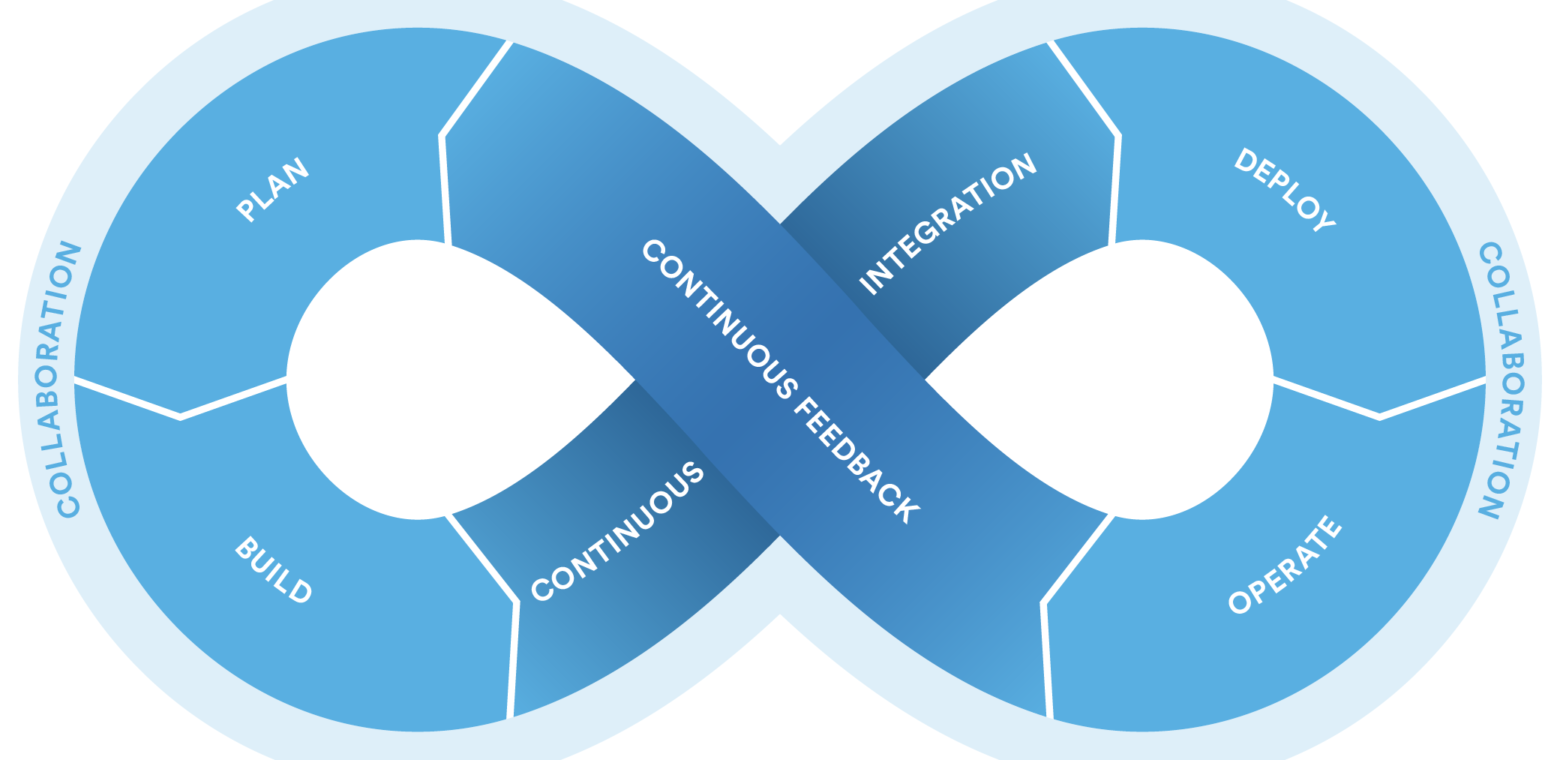
\includegraphics[width=13cm]{images/atlassian/atlassian-state-of-devops-report-2016-devopsloop.png}
    \caption{Atlassian DevOps loop}
    \label{fig:atlassian-state-of-devops-report-2016-devopsloop}
\end{figure}
% https://3kllhk1ibq34qk6sp3bhtox1-wpengine.netdna-ssl.com/wp-content/uploads/devopsloop-1560x760.png



\section{From conceptual models to practicalities}
The previous sections introduced five conceptual models that help to establish the context for the ecosystem, structural aspects of mobile apps and perspectives where mobile apps can be observed, analogue and digital feedback, usage analytics and DevOps considerations. The next five sections cover various practical aspects of mobile apps including development and usage lifecycles, information sources and finally choices for engaging with analytics.

\section{Mobile apps and development team's mobile devices}
A mobile app is more than compiled source code, it includes various resources such as text, images, audio, screen layouts, and sometimes other contents. Many include software libraries from one or more sources. Mobile apps are also digitally signed. Data and information can be obtained for these various constituent parts, for instance some failures may occur within a library at run-time and be reported in logs and via mobile analytics.

Development team's mobile devices, with occasional exceptions are often the same device models that end users have and use; and furthermore they have similar end-user accounts and the majority of their apps are installed in similar ways to those installed on end-user devices. These similarities have some important implications - data on the usage of these devices by the development team may also be collected and considered as being part of the end-user population, and any in-app analytics in the various installed apps may provide their data to the respective mobile analytics systems,~\emph{etc.}

These devices may be configured differently and they may also run local builds and internal releases of apps. The apps may be configured to provide different amounts of information in local logs and/or using mobile analytics libraries for instance to either distinguish the usage or to suppress data from being shared. Knowing and understanding these nuances can help interpret some of the sources of data and information pertaining to these devices and apps.

\section{Mobile app development lifecycle}
To provide some context for this section, Figure \ref{fig:ci-cd-development-and-feedback}~\footnote{Reproduced from \emph{``An empirical study of architecting for continuous delivery and deployment"}~\cite{shahin2019empirical_study_architecting_cd}}
illustrates a modern continuous software lifecycle including feedback. We can observe several distinct stages in the development and deployment of software and the feedback each stage can provide. %MUST-DO check the guidelines for reproducing and citing a figure as-is.
%
In contrast, Figure \ref{fig:google-play-app-development-and-feedback} illustrates a similar software lifecycle for Android apps released through Google Play together with the various forms of feedback~\footnote{Here we have excluded feedback from the app store, nonetheless it exists for many app stores.} 

Key differences between typical CI/CD lifecycles and the one for Google Play is the pre-launch testing and the app store providing both user feedback and a service called Android Vitals. The pre-launch reports are generated automatically by Google where the app store runs automated monkey testing on a farm of Android devices and various static analysis checks of releases deployed to any of the test channels. They are described in~\href{subsection-test-channels}{Test Channels}. %MUST-DO actually add information on the test channels and how releases can be promoted to production releases in Google Play.


\begin{figure}[htbp!]
    \centering
    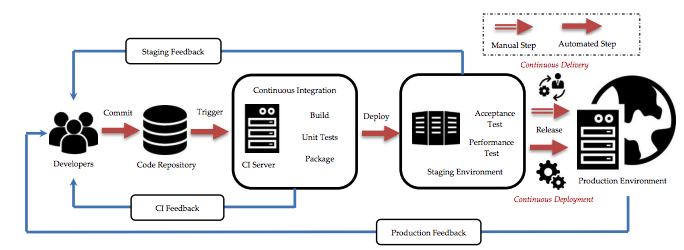
\includegraphics[width=13cm]{images/ci-cd-development-and-feedback.png}
    \caption{CI/CD development and feedback, reproduced from~\cite{shahin2019empirical_study_architecting_cd}}
    \label{fig:ci-cd-development-and-feedback}
\end{figure}

There are additional sources of \emph{analogue feedback} from people, including from alpha and beta testers and end users; and \emph{digital feedback} from Google tools and from usage data collected from the field. These terms are expanded in the section~\href{analogue-and-digital-feedback}{\emph{\nameref{analogue-and-digital-feedback}}}.

\begin{figure}[htbp!]
    \centering
    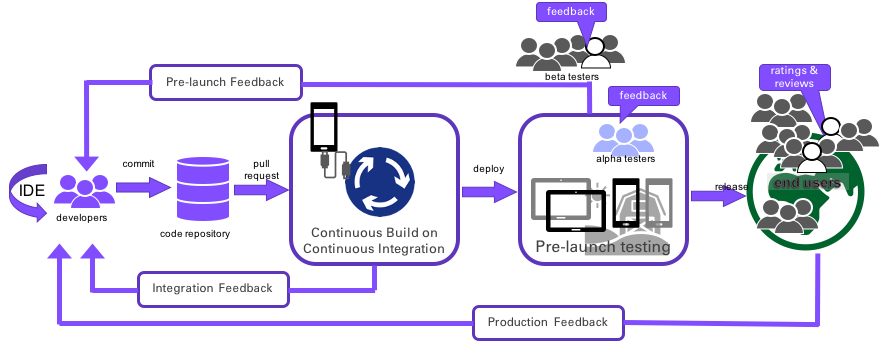
\includegraphics[width=13cm]{images/google-play-app-development.png}
    \caption{Google Play App Development and Feedback}
    \label{fig:google-play-app-development-and-feedback}
\end{figure}

\section{Mobile app usage lifecycle}
Mobile apps have a usage lifecycle, which starts when an app is chosen to be installed and ends with either abandonment or active removal of the app from a device. Figure~\ref{fig:mobile_app_usage_lifecycle}~\footnote{Based on a figure in~\cite{bohmer2011falling_asleep_with_angry_birds}} illustrates the possible stages of a mobile app's life on a user's device. Google Play Console collects data consistent with this lifecycle, analyses it and provides aggregate reports based on their analysis. 

For clarity and completeness there is another lifecycle when the app is running, described in the Android documentation as the \emph{``Processes and Application Lifecycle"}~\cite{android_processes_and_application_lifecycle} These are more detailed and are not included in the reports Google provides developers. %(I doubt their details would be recorded either). 
Note: the processes and application lifecycle may affect how in-app analytics libraries behave, including when they transmit their data to their respective central servers.

% More info and code samples: https://www.vogella.com/tutorials/AndroidLifeCycle/article.html

\begin{figure}[htbp!]
    \centering
    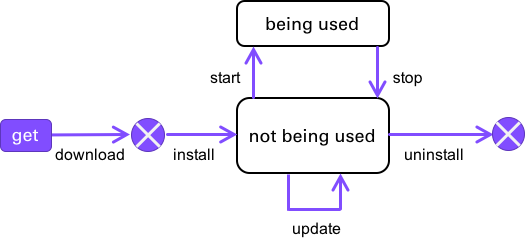
\includegraphics[width=12cm]{images/mobile_app_usage_lifecycle.png}
    \caption{Mobile App Usage Lifecycle}
    \label{fig:mobile_app_usage_lifecycle}
\end{figure}

A later section~\href{platform-level-analytics}{\emph{\nameref{platform-level-analytics}}} provides a proposal of how Google collects the underlying data (they do not document, explain or encourage research in how their system works, We return to their (Google's) reported behaviour and the effects later in this thesis). % MUST-DO add link to: Developers banned from app store ecosystem and their apps removed.
And the chapter \href{software-contributions-chapter}{\emph{\nameref{software-contributions-chapter}}} describes software we developed to help collect data from Google Play Console in order to facilitate both research and to enable developers to collect and use data...

Crashes are often considered a concrete measure of poor performance of software and there has been extensive research in crashes for Android applications, in particular. I suspect there are various reasons for the focus on crashes as an oracle for testing software, crashes are unambiguous (even if the causes are not) and they are also binary so easy to determine whether software has, or has not, crashed. 

In 2017, Google launched a service called Android Vitals as a new, intrinsic part of Google Play Console,~\cite{googblogs_I_O_2017_everything_new_in_the_google_play_console}, where they popularised a measure called \emph{Stability} to assess the quality of Android apps. Their measure includes both crashes and when an application freezes or is unresponsive for at least 5 seconds from a user's perspective, a term Google call Application Not Responding (ANR).


\subsection{DevOps for mobile apps}
This section starts with an overview of DevOps concept of an infinite loop for software generally before becoming more specialised on DevOps for mobile apps. %SHOULD-DO consider expanding this section. TBD how much I should write about the concepts and terms. 
The focus here is on data from various stages of a conceptual infinite combined development and operations process to indicate where mobile analytics applies in terms of providing data to the development team. This data includes: log data, static analysis results, test results, release and usage data, and mobile analytics data and reports.

In October 2020, one of the students taking part in the PhD symposium at the ICST2020 conference presented a variation of the DevOps loop (as illustrated earlier in this chapter in Figure~\ref{fig:atlassian-state-of-devops-report-2016-devopsloop}) that is relevant to this research. In the student's figure their focus was on crash reproduction and this illustration is temporarily illustrated in Figure~\ref{fig:crash-reproduction-icst2020}(~\emph{pending an update from the presenter of that topic}).

\begin{figure}[htbp!]
    \centering
    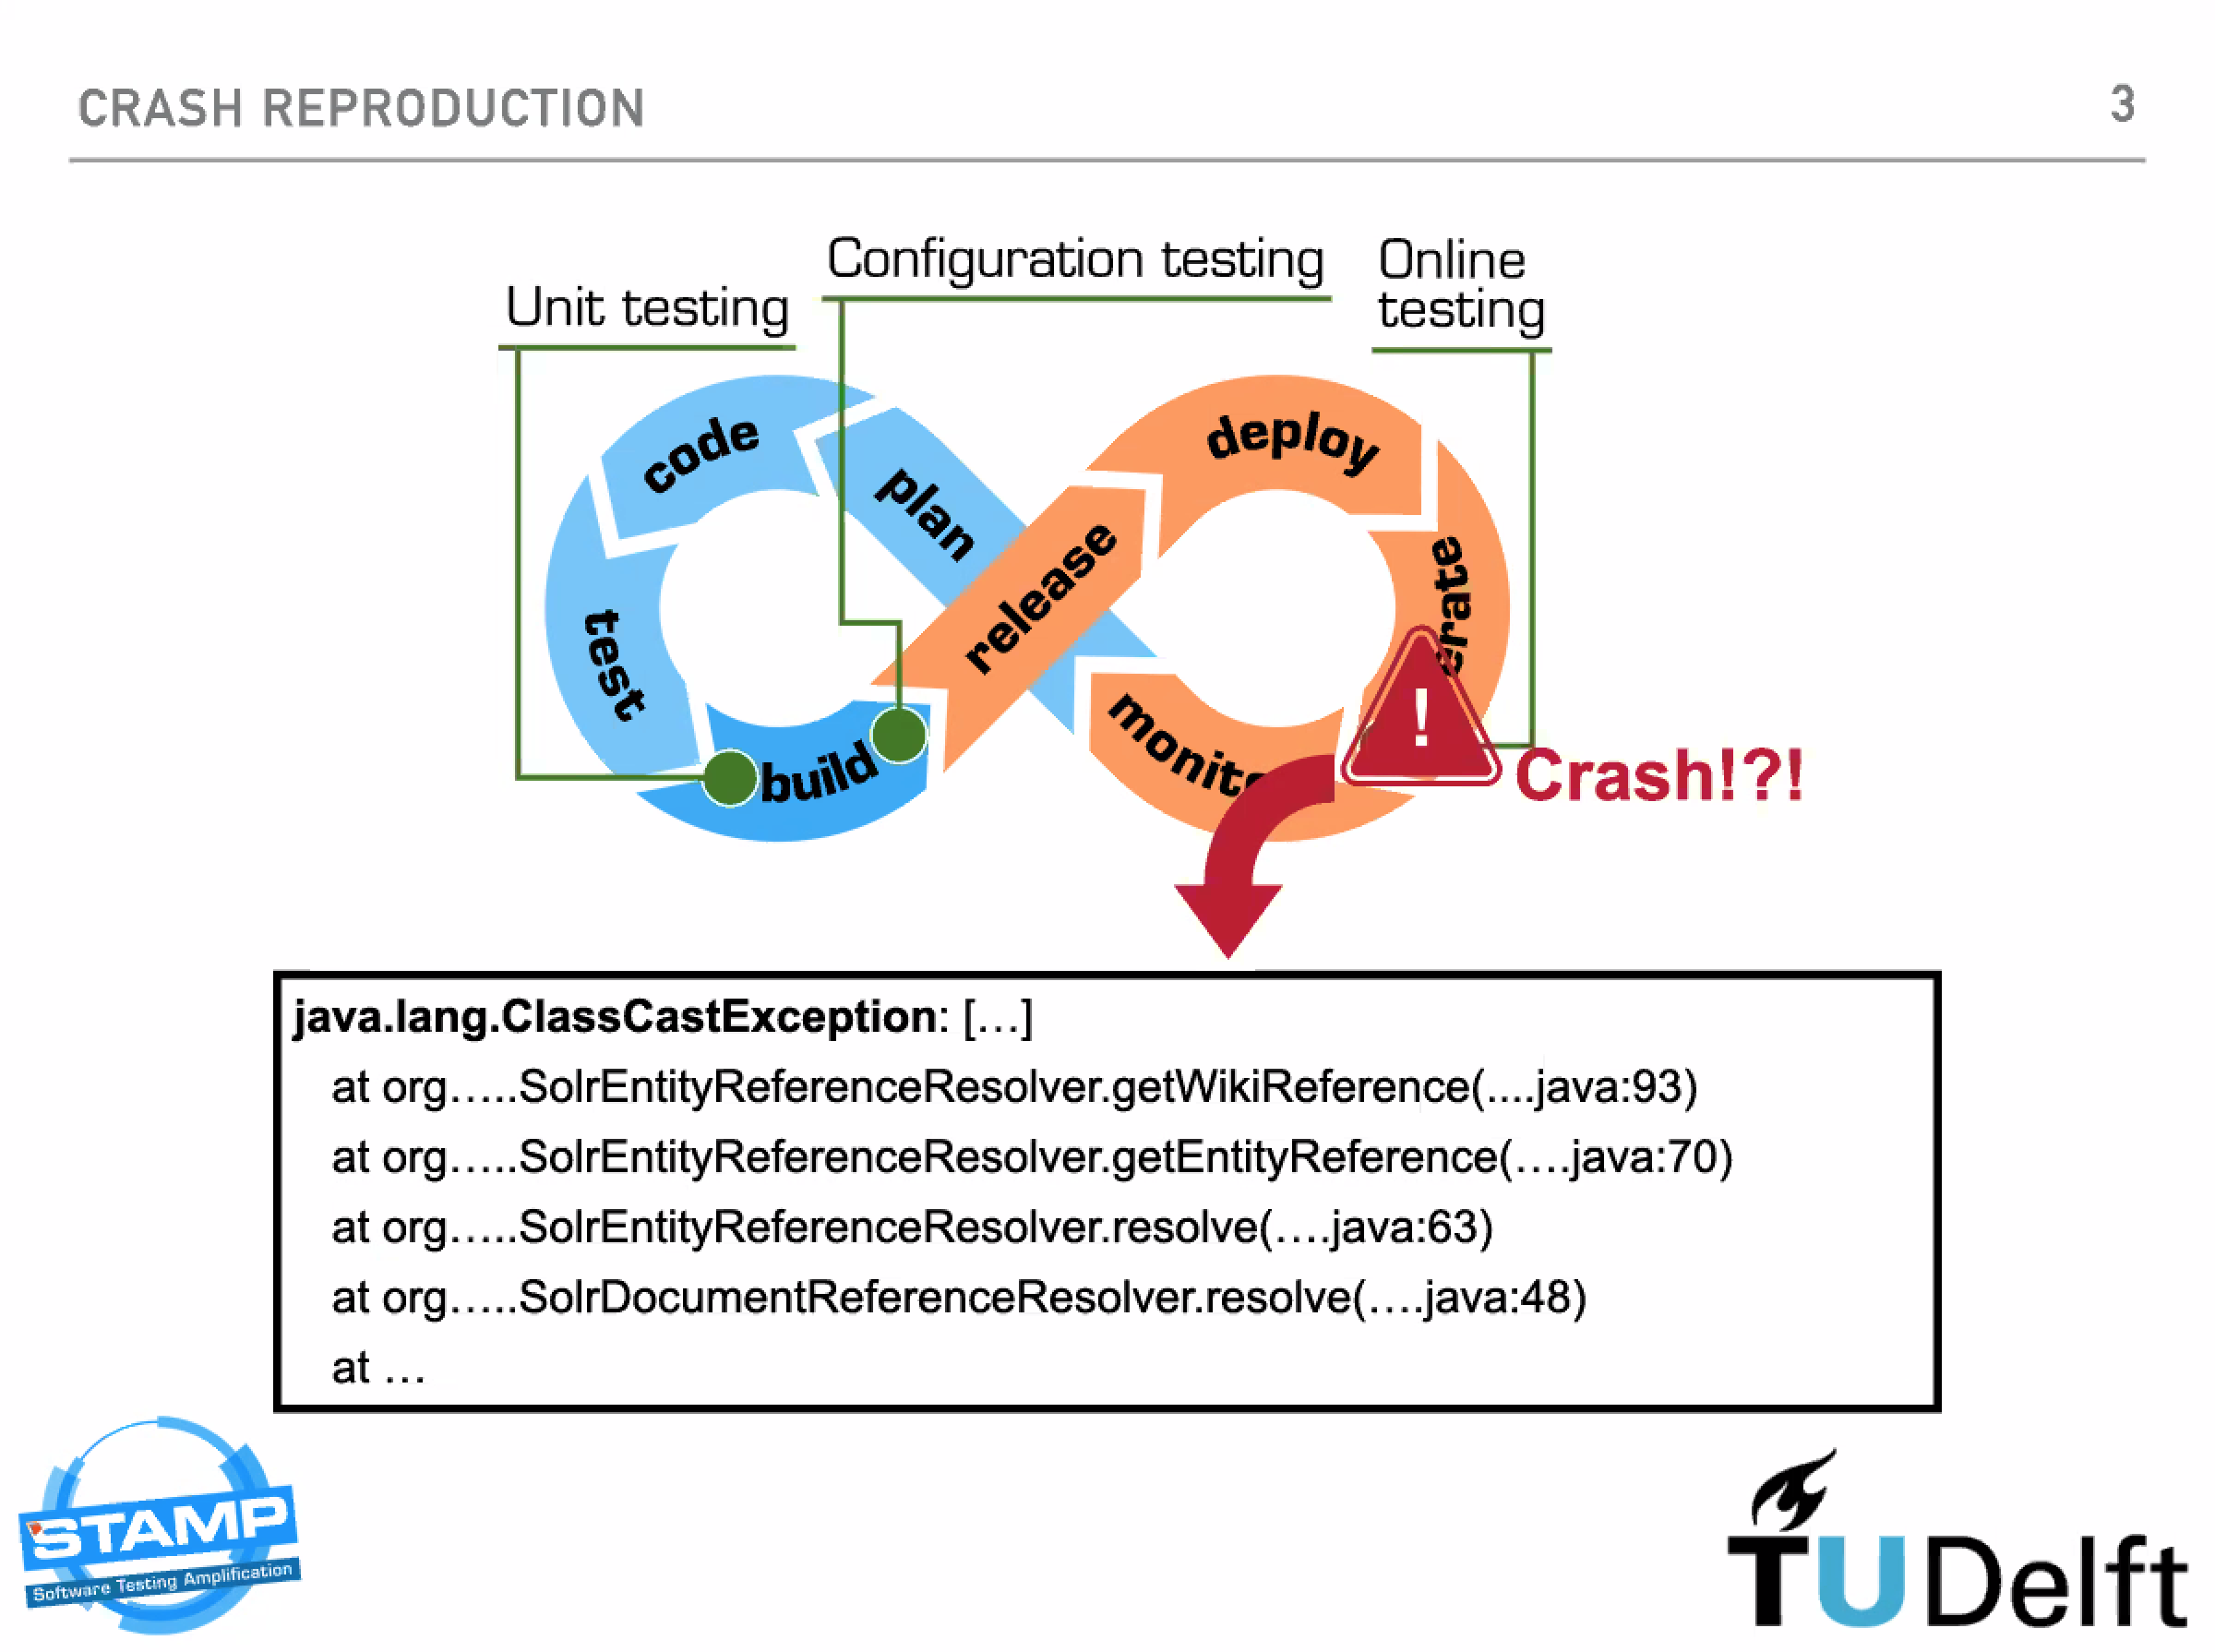
\includegraphics[width=14cm]{images/icst-2020/crash-reproduction-icst2020.png}
    \caption{Temporary image: Crash Reproduction}
    \label{fig:crash-reproduction-icst2020}
\end{figure}

Figure~\ref{fig:oberve-and-apply-devops-loop} is revised illustration that shows, in red, the extent software can be observed, and in green of when the results of those observations can be applied to the code. Note: the observations can be applied throughout every phase, for instance during deployment aberrant behaviour observed during the deployment may lead to the deployment being paused.

\begin{figure}[htbp!]
    \centering
    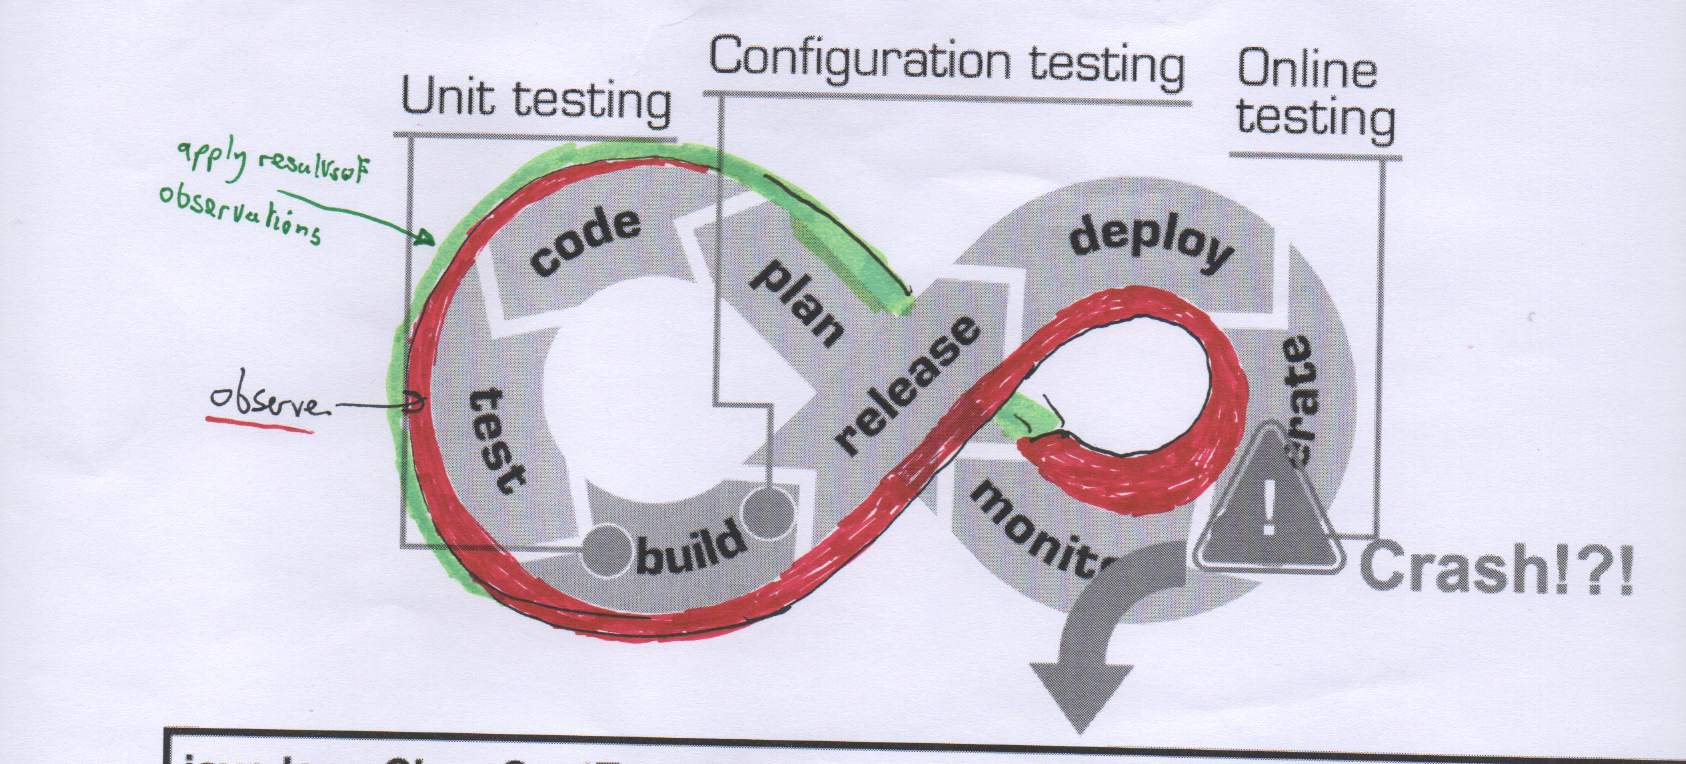
\includegraphics[width=14cm]{images/rough-sketches/hack-of-devops-crash-figure.png}
    \caption{Rough Sketch: Concept of feedback on software and applying it}
    \label{fig:oberve-and-apply-devops-loop}
\end{figure}

Data is available using various sources about software from the outset of coding until the software dies; however for the purposes of this thesis the focus is on when the software is actively used and maintained, as illustrated in the previous three figures:~\ref{fig:atlassian-state-of-devops-report-2016-devopsloop},~\ref{fig:crash-reproduction-icst2020},~\ref{fig:oberve-and-apply-devops-loop}. 

During coding code analysis tools such as static analysis identifies patterns of potential concern in the source code and similar artifacts such as GUI layouts, strings in resource files, and so so. Tests can also be created and performed from the outset of the coding to provide runtime feedback (~\emph{i.e.} data) about the software under test, and similarly developers can add logging statements and also use logging built into the operating system that both provide data that can be mined to learn about the software's behaviours.

The build process may include configuration details, for instance to create a range of custom applications, to include instrumentation, to compress and obfuscate the application binary, and to create debug and release editions of the software. Data about the build process and about what has been built may also be observed and analysed and the products tested and analysed; for example an application binary can be scanned for information leakage in an obfuscated build, and builds can be tested to provide more data about how the software performs.

The release and deployment phases will be covered in more detail in the next section; here the focus is on the data available as part of these phases. 

As software is released the software transitions from being within the view of the development team to being used by others where the development team no longer has direct access to the devices that have the app installed or being used. They are remote from the use of the app. This means that local access to devices (to see what's happening and to try things out) and to the device's logs are unlikely to be practical, other sources of information now need to take precedence.

The release of a mobile app using an app store is subject to the processes and controls applied by the provider of the app store. The app store may offer both free and paid-for optional services to the developer, for example Google provides optional, free pre-launch reports that contain the results of automated testing and static analysis of application binaries. The app store may provide reports to the development team particularly if they decide to delay or block a release or suspend an app from being downloaded by end-users.

Usage is the ultimate active phase for a mobile app installed on a user's device. Simplifying slightly, as some apps run automatically in the background, most apps are started and used by end-users. Aspects of the usage can be recorded by various software utilities, in particular by the platform which records when an app starts and when it terminates. The platform can also record when an app is installed, when it is updated, and when it is uninstalled. The app store may provide developers with reports and statistics on the app's install base and usage. The app store may also provide developers with information about the performance of the app including any failures of the app while it was running.

Crashes are logged locally by the platform, some platforms may also record other failures and performance related data as well as resource utilisation and various capacities such as battery level locally. The platform may have permission from end-users to forward a copy of the information logged locally on the device and to use it for various purposes.  

\subsection{Software releases for mobile apps}
For mobile apps, the release management may include deployment of the app to end-user's devices either as a fresh install for new users or as an update for existing users that app on a given device~\footnote{Mobile apps for Apple and Google app stores are installed per device and licensed per user so users can freely choose how many devices to install an app on, and they may even have different releases of the same app on different devices.}.

Releases may be acute or chronic in nature. Acute releases are actioned immediately and deployed as soon as practical. Chronic releases may involve alpha (closed-group membership) and beta (open-group membership) testing followed by rollout in stages, for instance starting at 10\% of the user-base, then increasing to 25\%, and so on until the new release is available to 100\% of the user-base. Note: there is no guarantee that the new release will be deployed to the entire user-base, and in my experience some users will keep using much older releases for as long as several years after newer releases were made available to them. 

The actual deployment and market penetration of a new release depends on several factors which may be outside the developer's direct control. This particularly applies for mobile apps made available through an app store where the app store and end-users can block new releases being applied. In my experience across a range of Android apps, for a 100\% rollouts it takes about a week for the new release to be installed on 50\% of the user-base's devices, however the range varies from 3 days to several weeks to reach 50\%.  

\begin{figure}[htbp!]
    \centering
    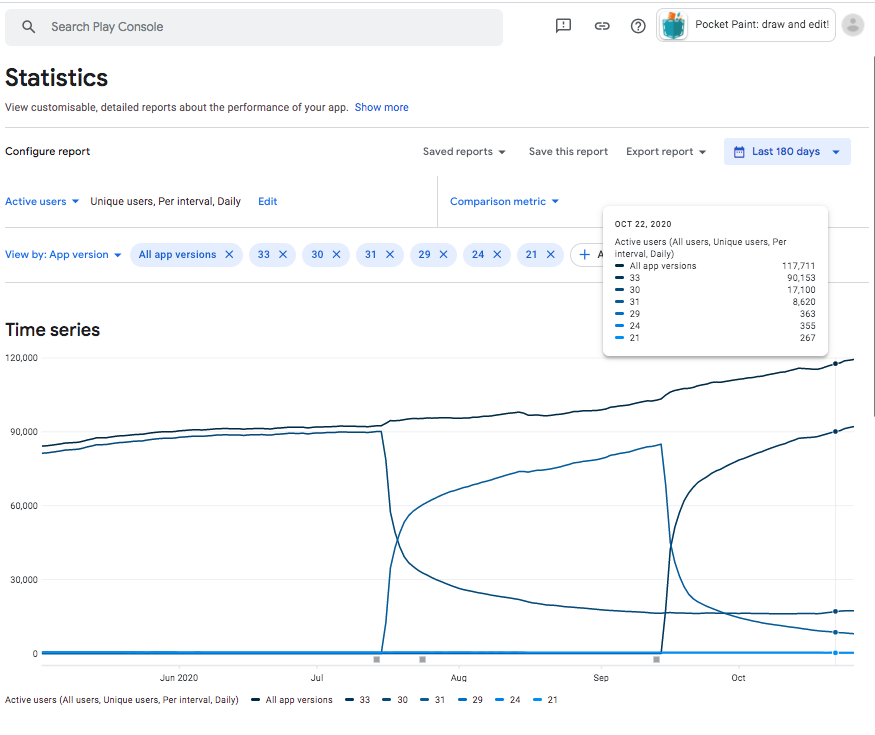
\includegraphics[width=15.5cm]{images/android-vitals-screenshots/PocketPaint-ActiveUsers-180days-2020-10-29.png}
    \caption{PocketPaint Active Users 180 days by app version}
    \label{fig:pocketpaint-180d-active-users}
\end{figure}

Figure~\ref{fig:pocketpaint-180d-active-users} illustrates a typical pattern of the majority of the userbase migrating from one app release to another and yet others remain with older releases during this period of 180 days (apologies for the small text in the image it was impractical to resize it adequately). Note: Google defines active users as:~\emph{``
The number of users who have your app installed on at least 1 device that has been turned on in the last 30 days"}~\footnote{Text extracted from the online help for the `Active users' contextual help icon in Figure~\ref{fig:pocketpaint-180d-active-users}.} so it's not necessarily those who use the app in this period. The residues of users who remain on older releases of the app constrains the rate of change of the overall statistics as measured by Google Play Console and Android Vitals. This means that old buggy releases may continue to adversely affect the overall stability metrics for the app for long periods, even for months and years. Conversely, the project team may have addressed some of the causes of poor stability yet don't have a viable way of proposing users upgrade to the newer releases, and sometimes newer releases may have undesirable features or characteristics from an end user's perspective.

\begin{figure}
    \centering
    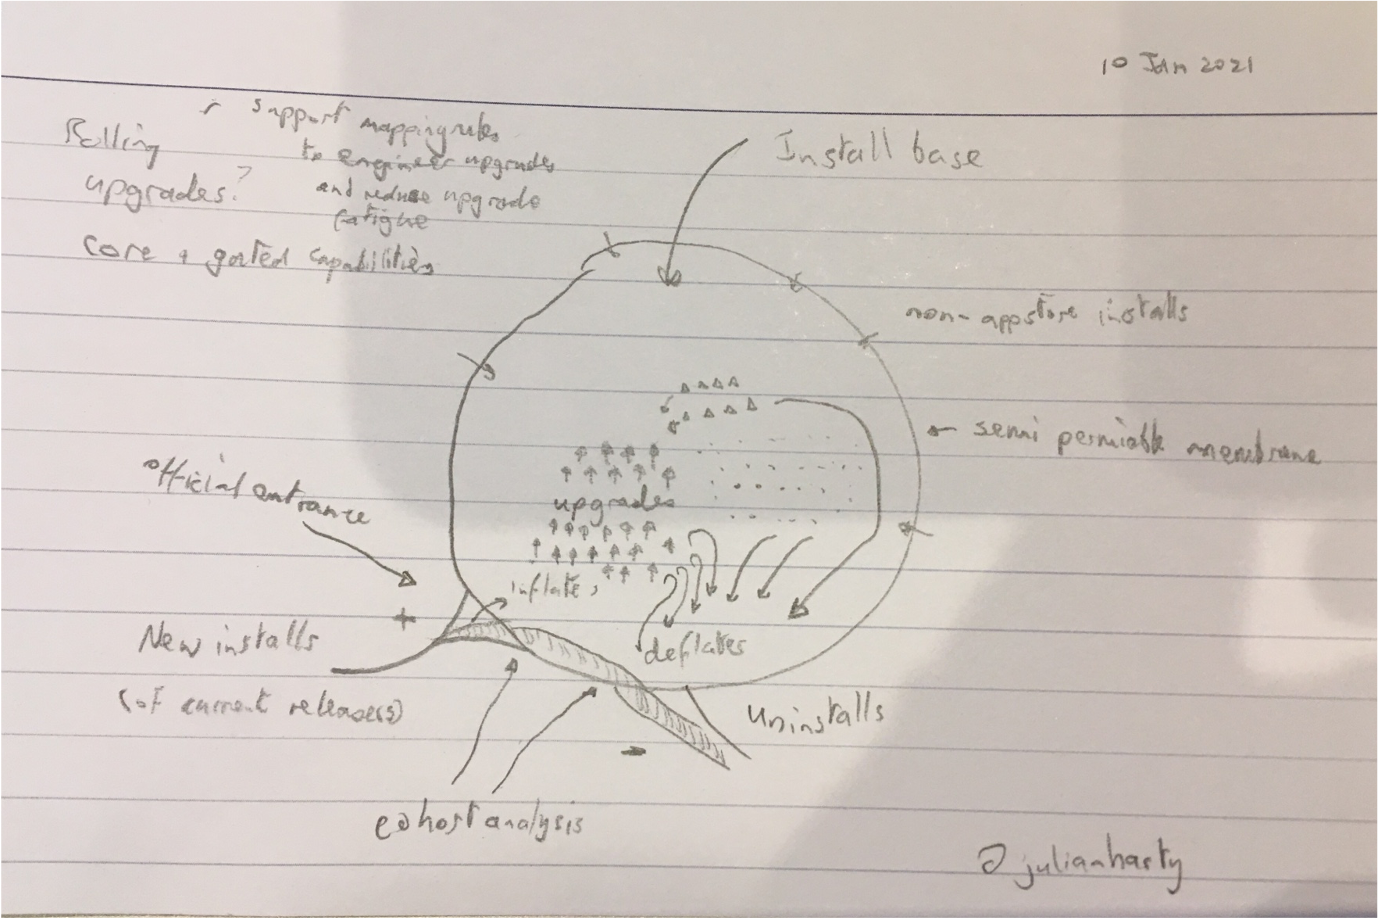
\includegraphics[width=14cm]{images/rough-sketches/app-install-base.png}
    \caption{App install base}
    \label{fig:app-install-base-rough}
\end{figure}

\textbf{Installation base}: The rough sketch in Figure~\ref{fig:app-install-base-rough} illustrates static and dynamic aspects of the installation base for a mobile app. The approximate circle contains the installation base for an app. The size ebbs and flows based on new installs - which inflate the shape, and uninstalls - which deflate it. In current mainstream app stores users do not get a choice of which release of an app they will receive when they receive it, that choice is made by the app store using one or more releases provided by the developer. The app store may allow developers to choose various criteria for current releases, such as a percentage rollout, and then apply that on behalf of the developer. The boundary may be considered semi-permeable as some installations are not sourced from the app store. A key consideration is that upgrades apply to the install base so they occur within a population and do not change the number of installs. That said they may lead to decreases in the installation base for various reasons. Some users may uninstall an app prompted by learning of a new update of the app - for instance if it requires permissions the user considers intrusive or unsafe; others may uninstall the app after the update, for instance if they believe it is too buggy to merit using. Note: they are not able to revert to an earlier release within the current major app store's practices / constraints. 

To sum up so far, new installs receive the most current release gated by the rollout algorithms implemented by and in the app store. Upgrades also receive the most current release gated by the same rollout algorithms.

\textbf{Cohorts}: represent a group of users who share something in common and measures at intervals through time. Examples include new users who install the app on a particular day or in a particular week. They are used in analysis, for instance to measure what proportion of new users still have the app installed a week later. Cohorts can also be used to group users with a distinct release of an app, and so on. Useful introductions to cohort analysis using Google Analytics are available online~\citep{codehouse2020_cohort_analysis, googleanalytics2021_the_cohort_analysis_report}, and cohorts are used in various analytics tools including Google Analytics and Firebase Analytics. 

% https://www.codehousegroup.com/insight-and-inspiration/digital-strategy/cohort-analysis-and-how-to-use-it-in-google-analytics
% CHEST journal: Cohort Studies https://doi.org/10.1016/j.chest.2020.03.014

One reason why users uninstall an app is because of poor quality behaviours by the app. In a survey by Dimensional Research, 3011 participants completed an electronic survey to identify key factors that led to end user satisfaction with mobile apps. The research also `... sought to determine what users did when they were unsatisfied with a mobile app.' (page 5). 
53\% of respondents have uninstalled or removed mobile apps that regularly crashed, stopped responding or had errors and 37\% stopped using the app (page 16)~\citep{dimensionalresearch2015_mobile_app_use_and_abandonment}~\footnote{The report is free of charge upon request: \url{https://techbeacon.com/resources/survey-mobile-app-users-report-failing-meet-user-expectations}}.

To sum up again, the installation base relies on a combination of existing and new users. Updates can lead to some existing users uninstalling the app - a topic to consider when planning releases of the app. Cohorts can be used to measure the effects of new releases of an app and several analytics tools already use them for tracking the retention of new users. Poor quality of an app may lead to more uses abandoning and even uninstalling the app. As a hypothesis: if an update of an app improves the quality of an app for a user the user may be pleased with the update and continue using the app, conversely if an update does not improve the quality of the app for that user some users will merely stop using the app others will actively deinstall it. Releases can be a point of inflection in terms of the userbase.

\textbf{Forced updates?} Some developers, and some platforms, may incorporate mechanisms to encourage or even try to force users to update their apps. However, doing so may upset and alienate some users. One of the case studies,~\href{section-greentech-apps}{\emph{\nameref{section-greentech-apps}}}, has used these mechanisms and this topic will be expanded in that case study. In contrast, the Kiwix Android app has over 70 releases being reported as active in a 7 day period, some several years old. Figure~\ref{fig:kiwix-30d-active-users} shows the overall active user base and the top ten of the 70+ releases according to Google Play Console~\footnote{Google Play Console limits the graph to ten items on the secondary category.}.

\begin{figure}[htbp!]
    \centering
    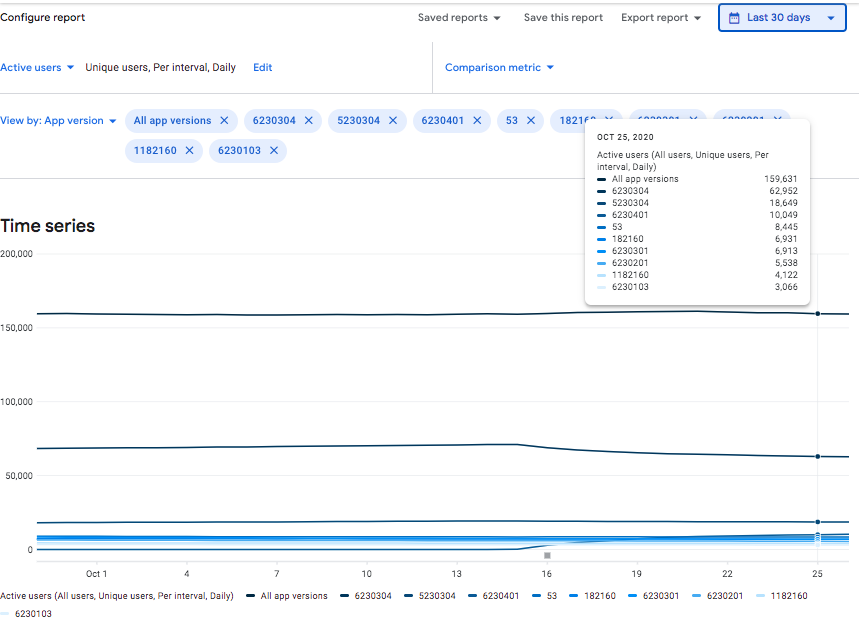
\includegraphics[width=15.5cm]{images/android-vitals-screenshots/kiwix-ActiveUsers-30-days-2020-10-29.png}
    \caption{Kiwix Android Active Users 30 days by app version}
    \label{fig:kiwix-30d-active-users}
\end{figure}

As mentioned above, there are various practical constraints to the frequency of releasing mobile apps using an app store. Chiefly there are two constraints: 1) the relatively slow rollout of new releases to the user-base which can take a week or more to achieve 50\% and also 2) the app store's review process which has been a hotly debated topic particularly by developers who may end up waiting days or even weeks for a release to be approved. Apple states~\emph{``Review times may vary by app. On average, 50\% of apps are reviewed in 24 hours and over 90\% are reviewed in 48 hours."} and Google informs developers in Google Play Console~\emph{``We're experiencing longer than usual review times
Due to adjusted work schedules at this time, you may experience longer than usual review times for your app."} ~\footnote{This message is on the \texttt{app-dashboard} page for each app in Google Play Console and only visible to authorised development team members}. Sophisticated development teams may find ways to alleviate these constraints, for instance by shipping code updates that are applied by a current release rather than by creating and releasing a new binary of the entire app.

Given the constraints that are faced by the vast majority of mobile app developers, of rollouts taking many days and of needing to cope with sometimes lengthy delays in app approvals. 

Mention poor behaviour and their effects on app approvals.

TODO Discuss limits on releasing often that lead to an adapted set of working practices, release frequencies, etc. Perhaps do so elsewhere in this thesis?


\section{Information sources for app developers}
Developers want and need to know how well their apps are performing from various perspectives such as: growth and adoption (\emph{``do we have more users and are they using the app [more] often?"}), users' ratings and reviews (\emph{``do they like our work?"} and in terms of quality (\emph{``does it perform well? is it fast and reliable?"}). 

\begin{figure}[htbp!]
    \centering
    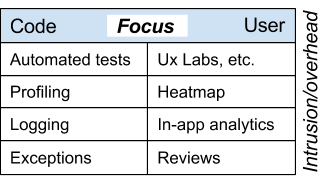
\includegraphics{images/ComparingTechniquesRHS.png}
    \caption{Comparing Techniques}
    \label{fig:comparing_techniques}
\end{figure}

\begin{table}[htbp!]
    \parbox{.40\linewidth}{
        \centering
        \small
        \begin{tabular}{lll}
            Technique  & Gen. Effort & Usage Effort  \\
            \hline
            Automated Tests  & High  & Medium \\ 
            Profiling   & 1 & 1 \\
            Code Quality tools & 1 & 1 \\
            Logging   & 1 & 1 \\ 
            Exceptions  & 1 & 1 \\ 

        \end{tabular}
        \caption{Focus: Code \label{HRVtable}}
    }
    \hfill
    \parbox{.40\linewidth}{
        \centering
        \small
        \begin{tabular}{ll}
            Technique & vector$_1$  \\
            \hline
            UX labs, etc. & 1  \\ 
            Heatmap & 1  \\ 
            In-app feedback & 1  \\ 
            App-store reviews & 1  \\
        \end{tabular}
        \caption{Focus: User \label{BACtable}}}
    \caption{Comparing techniques}
\end{table}

HRV data in Table \ref{HRVtable} and BAC data in Table \ref{BACtable}.

There are various techniques that can be used to assess aspects of quality of mobile apps. Figure \ref{fig:comparing_techniques} provides a visual overview of eight techniques. Of these four are code-oriented and the remaining four more user- or usage- oriented. They are ordered in approximate rank of the overhead, effort, or intrusion involved of each technique. % MUST-DO continue and expand this argument. Discuss why exceptions were chosen as one of the core elements of this research and PhD thesis.

Google's Google Play app store provides developers with answers to all these niggling questions through a developer-oriented user interface called Google Play Console. 
In Google Play Console they provide various tools, reports and data all aimed at informing developers about how their apps are 'doing' and performing. Broadly, these include an overview page with one line of pre-selected data per app managed by the Google Play \textit{Developer Account}. Then, per app, Google provides an overview dashboard of graphs which, in turn, link to more detailed reports and information which provide greater depth. (Examples are provided in the~\href{chapter-analytics-tools}{\emph{\nameref{chapter-analytics-tools}}} chapter.)  Some graphs only appear when Google's algorithms decide they are relevant, these seem to be related to events and/or volumes of underlying data.




\section{Passive, tacit, and explicit analytics choices}
Various degrees of choices are available depending on how actively the development team wishes to incorporate analytics into their development practices. These include using what already exists, where the data is gathered by others and made available to the developers, here these sources are called \emph{passive analytics}. Developers can choose to take more authority in the data collection, for instance by deciding what data they would like to collect and how they wish to collect it. They can use these tools at various depths, ranging from superficial use to actively maximising the efficacy of using analytics to provide them with the data they believe they need to achieve their outcomes. There is an interesting discussion in a blog article~\cite{mukherjee_implicit_versus_explicit_event_tracking_hits_and_misses} on what they term \emph{implicit, or codeless} and \emph{explicit or code-based} event tracking using web analytics tools. The article compares the benefits (hits) and flaws (misses) of both approaches. It also provides a flow chart to help teams select analytics tools that suit their context.

% More reading
% https://web.archive.org/web/20120401053907/http://www.wiikno.com/blog/explicit-vs-implicit-data
% MUST-DO check Patrick's recording of this webinar: https://snowplowanalytics.com/events/explicit-vs-implicit-tracking/ and write up germane items here.


\subsection{Passive Analytics}~\label{subsection-passive-analytics}
Passive analytics are those not actively under the control or influence of the development team, they are provided from other sources such as the operating system or the app store. In the context of this research the passive analytics are all managed by the app store, Google Play, and made available to developers through Google Play Console. As Google states in a US patent,~\emph{``several services provide passive analytics collection such as receiving information about the device type, time of usage, location usage, feature usage, and event reporting."}~\cite{googlepatent_hyman2016_collecting_application_usage_analytics}.  

% COULD-DO compare with the concept of passive monitoring https://en.wikipedia.org/wiki/Passive_monitoring however the Wikipedia article doesn't currently add enough to justify citing it or comparing with it.

\subsection{Tacit Analytics}~\label{subsection-tacit-analytics}
Tacit is variously defined as \emph{``Something tacit is implied or understood without question."}~\footnote{\url{https://www.vocabulary.com/dictionary/tacit}}, \emph{``Understood or implied without being stated."}~\footnote{\url{https://www.lexico.com/en/definition/tacit}, Note: Lexico.com is a new collaboration between Dictionary.com and Oxford University Press~\url{https://www.lexico.com/about}}, silent, wordless, or noiseless. 
%
It may be something that is inherent in the nature of using many of the third-party analytics libraries. In this research~\emph{tacit analytics} is where developers accept whatever default data is collected by an analytics library without the developer needing to do anything more than integrate the library into their app. 

\subsection{Explicit Analytics}~\label{subsection-explicit-analytics}
Explicit analytics is where developers have actively added code to interact with analytics libraries, for instance by calling methods in the API(s) provided by the library's. There are various degrees of use of the APIs and developers may have various intentions for calling these APIs.

\section{Drilling down into analytics}\label{section-drilling-down-into-analytics}
At the highest level of information, an item and an associated number provides some information: a total crash rate of 99.1 \%, 97K total installs, 37 reviews, and so on. These values may change over time, however if we do not keep track of previous values they cannot be compared, and also relevant information may be hidden behind the totals. The total sums up as many values as exist (from zero values onwards). Some of the reported analytics are of this high-level form.

Totals for subsets of the overall volume of data helps provide additional and potentially relevant information. Relevant subsets for mobile analytics include: date ranges, app releases, platform versions, and many others. Other examples, found in some analytics tools include crash clusters - collections of crash reports considered to be sufficiently similar to enable various individual crashes to be grouped and aggregated. The ability to segment and report on segments allows more detailed analysis than simply observing subsets. 

Comparisons with one or more peer groups provide relational analytics, helping answer: ``how is this app performing compared to various peer groups?" Unless the team has direct access to the data for their peer group, the statistics for the peer group need to be available to a trusted party who perform the comparisons. Some data is publicly available for instance the overall rating of an app together with a limited number of recent reviews and the total installs \textbf{MUST-DO} write up research that uses these sources in the related works chapter, add some of the citations here. There are also commercial services available, and some analytics tools, including Google Play Console, provide these comparisons as part of their services.

Individual records provide the most detail that's available. Note: Developers may be able to create new records and enhance existing records and/or add additional forms of analytics if they want/need more detail. Examples of individual records include stack traces for crashes and similar internal state data for ANRs. Some analytics tools allow developers to capture and subsequently see individual records, for instance details of an item added to an e-commerce shopping cart by an end user. Mobile analytics ultimately can only report on data that is provided to it. 

The analytics tool may or may not make aspects of the data available to the users of the tool. As a concrete example, Google Play Console provides developers access to individual reviews (with their associated rating), it also used to provide access to crashes and ANRs for several years before removing these and replacing them with summary data in 2018 \textbf{MUST-DO} add reference and cite it.

\textbf{MUST-DO} provide screenshots of category peer groups and custom peer groups. Discuss either here, or in a later chapter, Google's cap on the number of changes to the custom peer group.

Two key points in summary: being able to keep track of analytics as they change over time allows comparisons and trends to be determined. Additional detail can help identify meaningful differences for instance that a crash rate is much higher than the mean for a particular model of smartphone. 

How much information is needed to be actionable? (Thought: This may be more of a research question...)


\textbf{MUST-DO} introduce my concept of resolution.

\textbf{PERHAPS} introduce the concept of app peer groups here?


\section{Summary and transition}
% This chapter has introduced various concepts and topics which help provide context for the rest of this thesis. Some additional background material is available in various appendices, including more information on mobile analytics and various software contributions.
We now have a grounding in the domain of mobile apps, logging and mobile analytics which is underpinned by research in both academic research and grey literature. The next chapter describes the application of mobile analytics to software development practices for mobile apps.
